\documentclass[a4paper]{scrreprt}

\usepackage[german]{babel}
\usepackage[utf8]{inputenc}
\usepackage[T1]{fontenc}
\usepackage{ae}
\usepackage{amssymb}
\usepackage{graphicx}
\usepackage{hyperref}

\begin{document}

\title{BS Zusammenfassung}
\author{Benedict Hauck, Fedor Scholz\\Alex Tu, Florian Pohl}
\maketitle

\tableofcontents
\vspace{1cm}

\chapter{01aIntro}

\section{Was ist ein Betriebssystem?}
\begin{itemize}
	\item Vermittler zwischen Benutzer und Computer
	\item Ziele
		\begin{itemize}
			\item Benutzerprogramme ausfuehren und dem Benutzer das Loesen von Problemen erleichtern
			\item Computer benutzbarer machen
			\item Hardware des Computer effizient nutzen
			\item Benutzerziele
				\begin{itemize}
					\item Benutzbarkeit
					\item Einfach zu lernen
					\item Zuverlassigkeit
					\item Sicherheit
					\item Schnelligkeit
				\end{itemize}
			\item Systemziele
				\begin{itemize}
					\item Leicht zu designen, implementieren und unterhalten
					\item Flexibilitaet
					\item Zuverlaessigkeit
					\item Fehlerfreiheit
					\item Effizienz
				\end{itemize}
		\end{itemize}
	\item Vier Komponenten eines Computersystems in richtiger Reihenfolge
		\begin{itemize}
			\item Benutzer
			\item System- und Anwendungsprogramme
			\item Betriebssystem
			\item Hardware
		\end{itemize}
	\item Betriebssysteme verteilen Ressourcen
		\begin{itemize}
			\item Verwaltung aller Ressourcen
			\item Entscheidung bei konfligierenden Anfragen fuer effizientes und faires Benutzen der Ressourcen
		\end{itemize}
	\item Betriebssysteme kontrollieren
		\begin{itemize}
			\item Kontrolle der Ausfuehrung von Programmen, um Fehler und Missbrauch des Computers zu verhindern
		\end{itemize}
	\item Immer laufendes Programm ist Kernel, Rest ist System- oder Anwendungsprogramm
	\item Bootstrap program wird beim Starten/Neustarten geladen
		\begin{itemize}
			\item In ROM, EPROM oder FLASH als firmware gespeichert
			\item Initialisiert alle Aspekte des Systems, insbesondere die HW-Komponenten
			\item Laedt den Kernel und startet die Ausfuehrung
		\end{itemize}
\end{itemize}

\section{Organisation}
\begin{itemize}
	\item CPUs und device controllers sind fuer Zugriff auf shared memory ueber Bus verbunden
	\item I/O-Geraete und CPU koennen gleichzeitig ausfuehren
	\item Jeder device controller ist zustaendig fuer einen Geraetetypen
	\item Jeder device controller hat einen lokalen Puffer
	\item CPU bewegt Daten vom/zum Hauptspeicher zu/von lokalen Puffern
	\item I/O ist vom Geraet zum lokalen Puffer des controllers
	\item device controller informiert CPU per interrupts, wenn er fertig ist
\end{itemize}


\section{Interrupts}
\subsection{Haeufige Funktionen von Interrupts}
\begin{itemize}
	\item interrupt gibt Kontrolle an interrupt service routine ueber einen interrupt vector, welcher die Adressen von allen service routines beinhaltet
	\item interrupt architecture muss Adresse der unterbrochenen Intruktion speichern
	\item Einkommende interrupts sind aus, wenn gerade ein anderer bearbeitet wird, um lost interrupts zu verhindern
	\item trap ist ein interrupt, welcher von Software verursacht wurde (wegen eines Fehler oder durch eine Nutzer)
	\item Betriebssysteme sind interrupt driven
\end{itemize}

\subsection{Time interrupts}
\begin{itemize}
	\item Time interrupts um endlose Schleifen und Prozesse zu verhindern
	\item Wird nach bestimmter Zeitspanne ausgefuehrt
	\item Wird vor dem schedulen des Programm aufgesetzt
	\item Eingebettete Systeme haben Watchdog, welcher bis 0 zaehlt und dann resettet
\end{itemize}

\subsection{Interrupt Handling}
\begin{itemize}
	\item Betriebssystem merkt sich Status der CPU, indem es Register und Programmzaehler speichert
	\item Legt Typ des interrupts fest
		\begin{itemize}
			\item polling
			\item vectored interrupt system
		\end{itemize}
\end{itemize}

\section{I/O Struktur}
\subsection{Synchrone oder blockende I/O}
\begin{itemize}
	\item Nachdem I/O beginnt, geht die Kontrolle erst nach Fertigstellung der I/O wieder zum Benutzerprogramm
	\item Wait instruction laesst die CPU idlen
	\item Meistens nur ein I/O Request gleichzeitig
	\item Polling
	\item Signal
	\item Callback function
\end{itemize}

\subsection{Direct Memory Access Structure}
\begin{itemize}
	\item Fuer high-speed I/O, damit diese mit fast der Geschwindigkeit des Hauptspeichers Informationen uebertragen koennen
	\item Device Controller uebertraegt Daten in Bloecken vom Puffer direkt in den Hauptspeicher ohne CPU Eingriff
	\item Nur ein interrupt pro Block
\end{itemize}

\begin{figure}[ht]
\centering
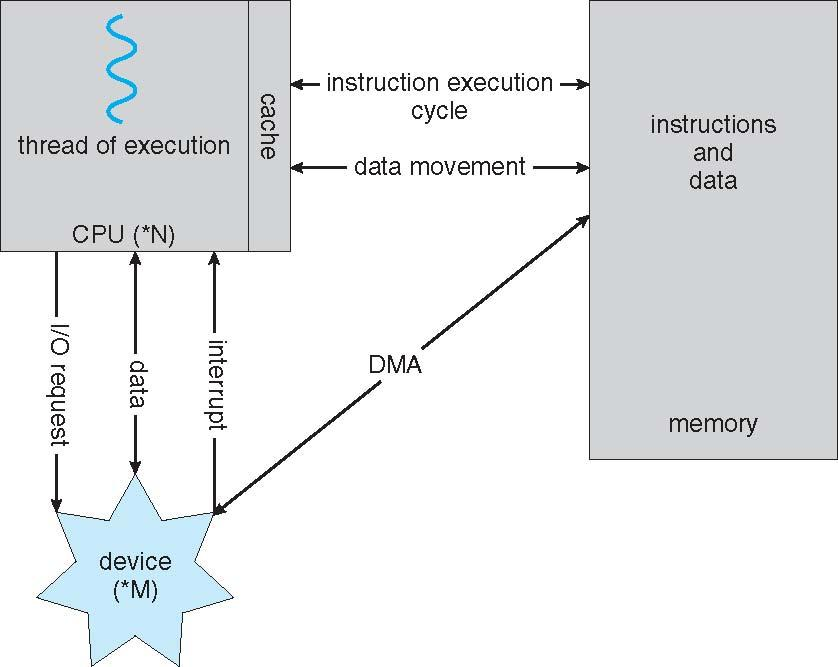
\includegraphics[scale=0.4]{dma.png}
\caption{Direct Memory Access}
\end{figure}

\section{Computer-System Architektur}
\subsection{Multiprozessor-Systeme}
\begin{itemize}
	\item Auch parallel systems, tightly-coupled systems
	\item Vorteile
		\begin{itemize}
			\item Erhoehter Durchsatz
			\item Wirtschaftlichkeit durch große Serie
			\item Erhoehte Zuverlaessigkeit - Fehlertoleranz
		\end{itemize}
	\item Zwei Typen
		\begin{itemize}
			\item Asymmetrische Mehrfachprozessorarchitektur
			\item Symmetrische Mehrfachprozessorarchitektur
		\end{itemize}
	\item Typen von Multiprozessoren
		\begin{itemize}
			\item Multi-socket systems
			\item Multi-Chip Module (MCM) (=Multi-Core)
			\item Chip Multiprocessor (CMP) (=Multi-Core)
			\item Simultaneous MultiThreading Processor (SMT)
		\end{itemize}
\end{itemize}

\subsection{Geclusterte Systeme}
Wie Multiprozessorsystem, nur dass mehrere Systeme zusammen arbeiten

\begin{itemize}
	\item Teilen sich meistens Speicher ueber storage-area network (SAN)
	\item Ermoeglicht hochverfuegbare Services, welche Fehler ueberleben
		\begin{itemize}
			\item Asymmetrisches Clustern hat eine Maschine im hot-standby mode
			\item Symmetrisches Clustern hat viele Maschinen mit laufenden Programmen, welche sich gegenseitig beobachten
			\item Manche sind fuer hochperfomantes computing (HPC)
		\end{itemize}
\end{itemize}

\section{Betriebssystem Struktur}
\begin{itemize}
	\item Multiprogramming ist noetig fuer Effizienz
		\begin{itemize}
			\item Einzelner Benutzer kann nicht CPU und I/O die ganze Zeit auslasten
			\item Multiprogramming organisiert jobs, sodass CPU immer beschaeftigt ist
			\item Untermenge aller Jobs ist im Hauptspeicher
			\item Einer wird ausgewaehlt per job scheduling
			\item Wenn dieser warten muss, wechselt OS den job
		\end{itemize}
	\item Timesharing (multitasking) laesst CPU so schnell jobs wechseln, sodass interaktives computing moeglich ist
		\begin{itemize}
			\item Response time < 1 Sekunde
			\item Jeder Benutzer hat mindestens 1 Programm im Speicher, welches ausgefuehrt wird $\Rightarrow$ process
			\item Wenn mehrere jobs bereit sind $\Rightarrow$ CPU scheduling
			\item Wenn Prozess nicht in Speicher passt $\Rightarrow$ swapping
			\item Virtueller Speicher erlaubt Ausfuehrung von Prozessen nicht komplett im Speicher
		\end{itemize}
\end{itemize}

\section{Uebergang vom User zum Kernel Mode}
\begin{itemize}
	\item Interrupt gesteuert durch Hardware
	\item Softwarefehler oder Anfrage erzeugt exception oder trap
	\item Dual-mode erlaubt es OS, sich und andere Komponenten zu schuetzen
	\item Mode bit bereitgestellt durch HW
		\begin{itemize}
			\item Zeigt an, ob System im User oder Kernel Mode ist
			\item Manche previligierten Instruktionen sind nur im Kernel Mode moeglich
			\item System call aendert Modus zu Kernel, Wiederkehr vom call aendert Modus zu User
		\end{itemize}
\end{itemize}

\section{Prozessverwaltung}
\begin{itemize}
	\item Prozess ist ein Programm waehrend der Ausfuehrung: Programm ist eine passive, Prozess eine aktive Einheit
	\item Prozessbeedigung erfordert das Freigeben von genutzten Ressourcen
	\item Single-threaded process hat einen program counter und wird sequentiell ausgefuehrt
	\item Multi-threaded process hat einen program counter pro thread
	\item Das Betriebssystem ist dabei fuer folgendes zustaendig:
		\begin{itemize}
			\item Erschaffen und loeschen von Benutzer- und Systemprozessen
			\item Suspenden und resumen von Prozessen
			\item Bereitstellung von Mechanismen fuer Prozessynchronisation
			\item Bereitstellung von Mechanismen fuer Prozesskommunikation
			\item Bereitstellung von Mechanismen fuer das Behandeln von deadlocks
		\end{itemize}
\end{itemize}

\section{Speicher}
\subsection{Storage Structure}
\begin{itemize}
	\item Hauptspeicher - großer Speicher, auf welchen CPU direkt zugreifen kann
	\item Zweitspeicher - Erweiterung des Hauptspeichers, welcher groß und nicht fluechtig ist
	\item Magnetische Disks - Oberflaeche in tracks geteilt, welche wiederum aus Sektoren bestehen
\end{itemize}

\subsection{Speicherverwaltung}
\begin{itemize}
	\item Alle Daten muessen vor und nach Verarbeitung im Speicher sein
	\item Alle Instruktionen muessen in der Reihenfolge ihrer Ausfuehrung im Speicher sein
	\item Aktivitaeten des OS
		\begin{itemize}
			\item Darauf achten, wer was im Speicher benutzt
			\item Bestimmen, welche Prozesse und Daten in und aus dem Speicher gehen
			\item Zuteilen und freigeben von Speicherplatz
			\item Einheitlichen, logischen Ueberblick bieten
				\begin{itemize}
					\item Abstrahiert physikalischen Eigenschaften zu logischen Einheiten: Dateien
					\item Jedes Medium wird von einem device kontrolliert
				\end{itemize}
		\end{itemize}
	\item Dateisystemverwaltung
		\begin{itemize}
			\item Dateien haeufig in Ordner organisiert
			\item Kontrolle ueber Zugriff
			\item Aktivitaeten des OS
				\begin{itemize}
					\item Erstellen und Loeschen von Dateien und Ordnern
					\item Grundsaetzliche Moeglichkeiten zum manipulieren von Dateien und Ordnern
					\item Abbilden von Dateien in sekundaere Speicher
					\item Sichern von Dateien auf nichtfluechtige Speicher
				\end{itemize}
		\end{itemize}
\end{itemize}

\subsection{Speicherhierarchie}
Die Speicherhierarchie haengt von folgenden Punkten ab:
\begin{itemize}
	\item Geschwindigkeit
	\item Kosten
	\item Fluechtigkeit
\end{itemize}

\begin{figure}[ht]
\centering
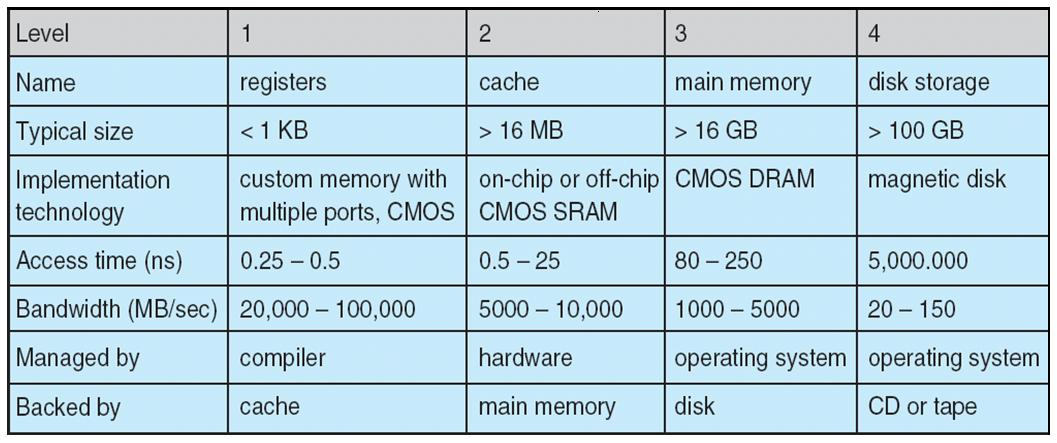
\includegraphics[scale=0.4]{storage.png}
\caption{Unterschiedliche Speicher und ihre Werte}
\end{figure}

\subsection{Caching}
\begin{itemize}
	\item Wichtiges Prinzip, taucht immer wieder auf (HW, OS, SW)
	\item Benutzte Information wird temporaer von langsameren zu schnelleren Speichern bewegt
	\item Zuerst wird im schnellen Speicher nach Information gesucht
		\begin{itemize}
			\item Wird sie gefunden, wird sie direkt benutzt
			\item Ansonsten wird sie in Cache kopiert und dort benutzt
		\end{itemize}
	\item Cache ist kleiner als Speicher, welcher gecached wird
\end{itemize}

\section{I/O Subsystem}
\begin{itemize}
	\item Betriebssysteme verstecken Eigenheiten der HW vor dem Nutzer
	\item I/O Subsystem ist verantwortlich fuer
		\begin{itemize}
			\item Speicherverwaltung der I/O inklusive Puffern, Cachen, Spoolen
			\item generelle Geraetetreiber-Schnittstelle
			\item Treiber fuer bestimmte Hardwaregeraete
		\end{itemize}
\end{itemize}

\section{Schutz und Sicherheit}
\begin{itemize}
	\item Schutz - Jeder Mechanismus, welcher den Zugriff von Prozessen und Nutzern auf Ressourcen kontrolliert
	\item Sicherheit - Verteildigung des System gegen interne und externe Attacken
	\item Systeme unterscheiden meistens zunaechst nach Nutzer
		\begin{itemize}
			\item Nutzeridentitaeten (user IDs) behinhalten Namen und Nummer
			\item User ID ist mit allen Dateien und Prozessen verknuepft, auf die der Nutzer zugreifen darf
			\item Gruppenidentitaeten (group IDs) erlauben den Zugriff einer Menge von Benutzern
			\item Privilege escalation erlaubt es Nutzern, die ID zu wechseln
		\end{itemize}
\end{itemize}

\begin{figure}[ht]
\centering
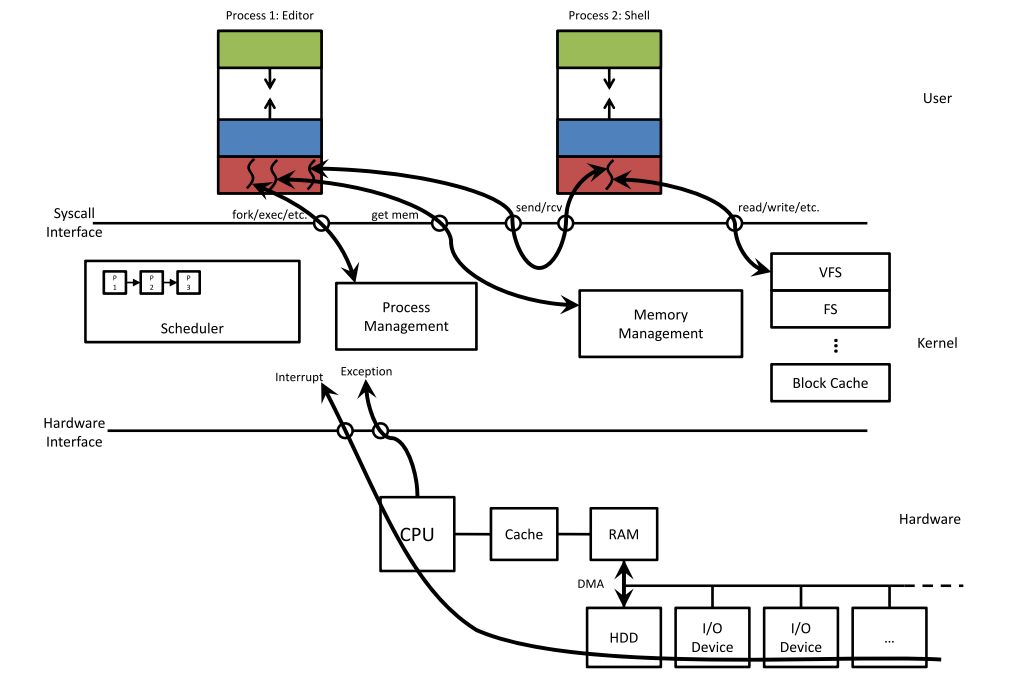
\includegraphics[scale=0.5]{big_picture.png}
\caption{Uebersicht}
\end{figure}

\section{Design und Implementierung von OS}
\begin{itemize}
	\item Policy: Was wird getan?
	\item Mechanism: Wie wird es getan?
\end{itemize}

\section{OS Service}
\begin{itemize}
	\item Benutzerschnittstelle (CLI, GUI, Batch)
	\item Programmausfuehrung
	\item I/O Operationen
	\item Dateisystemmanipulationen
	\item Kommunikation: Prozesse tauschen Informationen aus (shared memory oder message passing)
	\item Fehlererkennung
		\begin{itemize}
			\item Findet in CPU, Speicher, I/O Geraeten und Benutzerprogrammen statt
			\item Fuer jeden Typ von Fehler, hat das OS definierte Aktionen
			\item Debugmoeglichkeiten erhoehen Effizienz des Nutzen
		\end{itemize}
	\item Ressourcenallokation: s.o.
	\item Accouting: Welcher Nutzer nutzt wieviel?
	\item Schutz und Sicherheit: Besitzer von Informationen wollen Kontrolle ueber ihre Benutzung, Prozesse sollen nicht interferieren
		\begin{itemize}
			\item Schutz: Jeder Zugriff auf das System wird kontrolliert
			\item Sicherheit: Authentifikation
		\end{itemize}
\end{itemize}

\begin{figure}[ht]
\centering
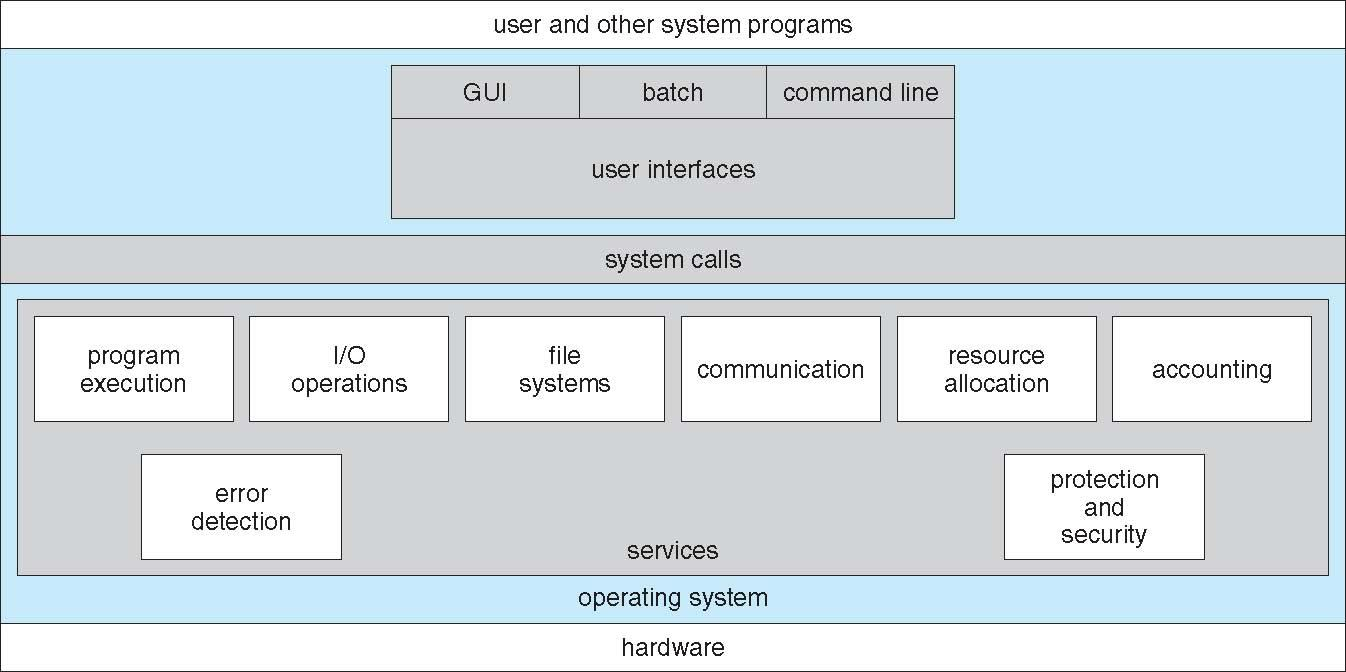
\includegraphics[scale=0.35]{services.png}
\caption{Ort der Services}
\end{figure}

\subsection{System Calls}
\begin{itemize}
	\item Schnittstelle zu den Services vom OS
	\item Meistens in hoeherer Sprache geschrieben
	\item Meistens ueber ein Application Program Interface (API) genutzt
	\item Win32 API, POSIX API, Java API
\end{itemize}

\begin{figure}[ht]
\centering
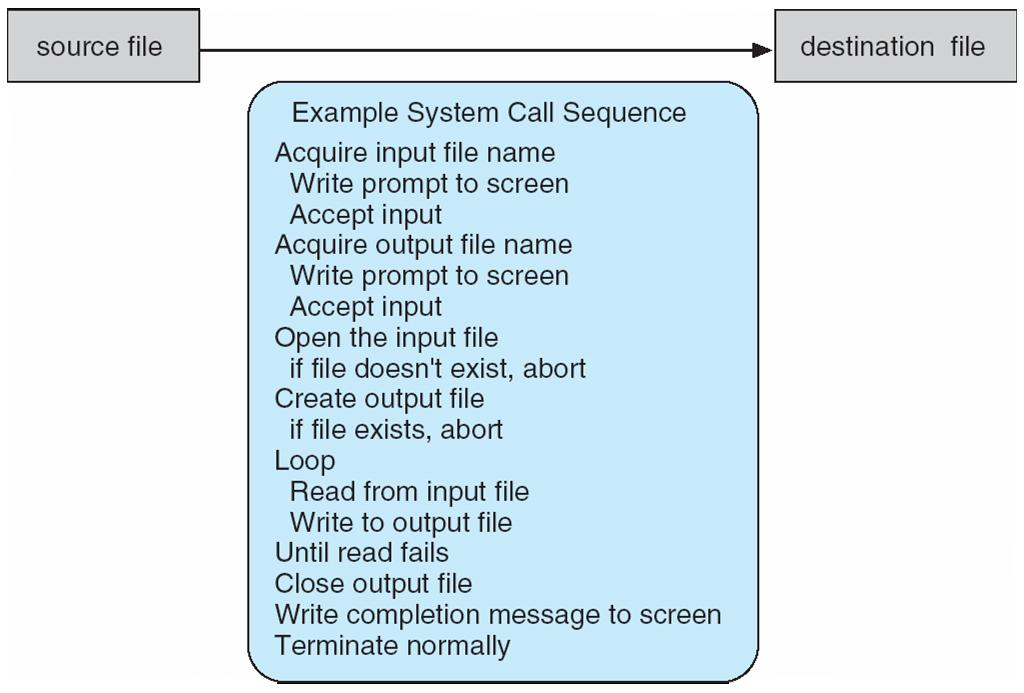
\includegraphics[scale=0.3]{system_call.png}
\caption{Aufrufsequenz eines Syscalls}
\end{figure}

\subsubsection{Beispiel fuer API}

ReadFile() Funktion in der Win32 API zum Lesen einer Datei:\\

\begin{figure}[ht]
\centering
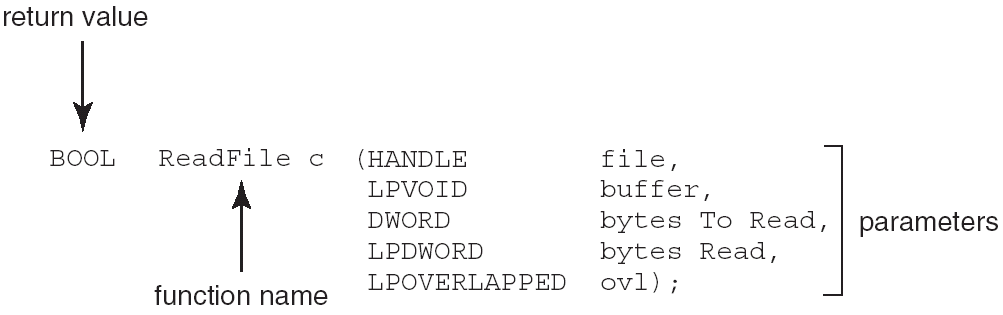
\includegraphics[scale=0.4]{api.png}
\caption{Head von ReadFile()}
\end{figure}

\begin{itemize}
	\item HAND: Zu lesende Datei
	\item LPVOID: Puffer, in den die Datei gelesen wird
	\item DWORD: Anzahl der zu lesenden Bytes
	\item LPDWORD: Anzahl der bereits gelesen Bytes
	\item LPOVERLAPPED: Gibt an, ob ueberlappende I/O genutzt wird
\end{itemize}

\subsubsection{Implementierung der System Calls}
\begin{itemize}
	\item Fuer jeden System Call gibt es eine Nummer
	\item System Call Schnittstelle veranlasst einen System Call im OS Kernel und gibt den Status sowie die Rueckgabewerte zurueck
	\item Aufrufer braucht nichts ueber die Implementierung zu wissen
\end{itemize}

\begin{figure}[ht]
\centering
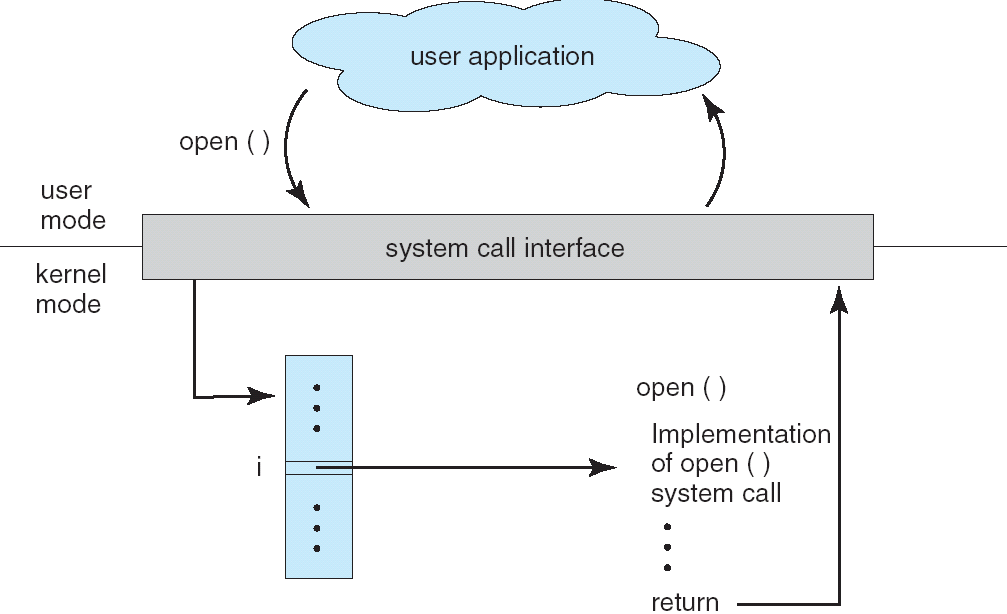
\includegraphics[scale=0.4]{syscall_os_relationship.png}
\caption{Beziehung zwischen Syscalls und OS}
\end{figure}

\subsubsection{Beispiel fuer C Bibliothek}

\begin{figure}[ht]
\centering
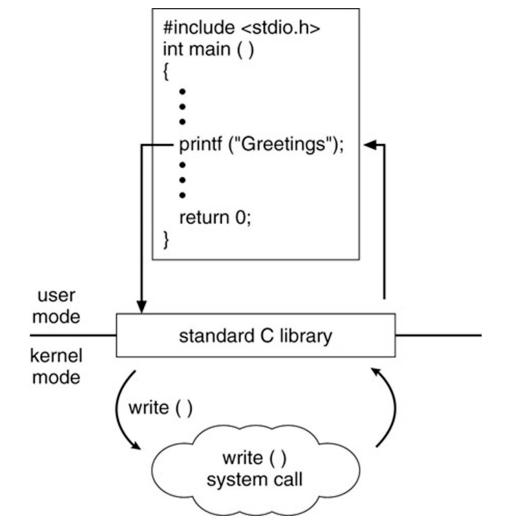
\includegraphics[scale=0.4]{printf.png}
\caption{Aufruf von printf}
\end{figure}

\subsubsection{Parameter}
Generell gibt es drei Methoden, Parameter an das OS zu uebergeben:
\begin{itemize}
	\item Durch Register, manchmal gibt es aber mehr Parameter als Register
	\item Durch einen Block, wobei seine Adresse ueber Register uebergeben wird
	\item Durch Pushen auf den Stack
\end{itemize}

\subsubsection{System Calls von Windows und Unix}
\begin{figure}[ht]
\centering
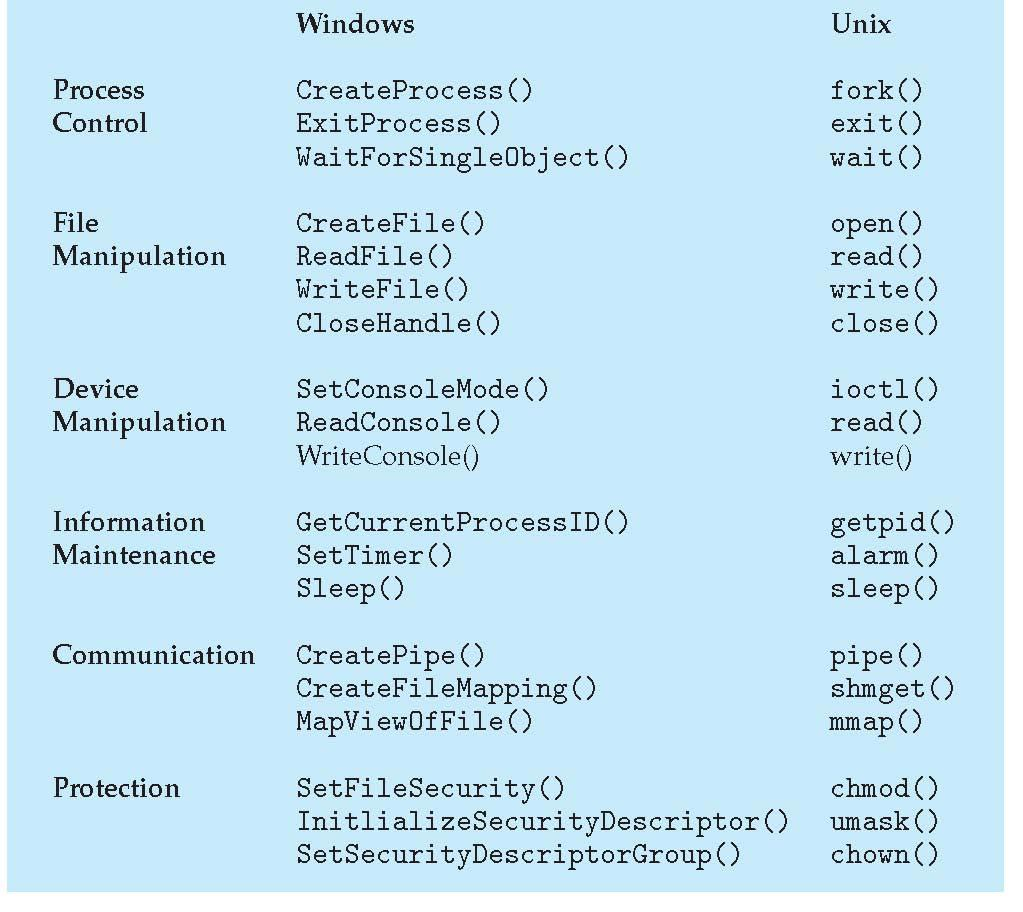
\includegraphics[scale=0.3]{syscall_examples.png}
\caption{Beispiele von Syscalls}
\end{figure}

\subsection{System Programs}
Systemprogramme ermoeglichen angenehme Umgebung fuer Programmentwicklung und -ausfuehrung:
\begin{itemize}
	\item Dateimanipulation
	\item Statusinformationen
	\item Dateimodifikation
	\item Support fuer Programmiersprachen
	\item Laden und Ausfuehren von Programmen
	\item Kommunikation
	\item Applikationen
\end{itemize}
Meisten geht die Sicht des Benutzer ueber Systemprogramme anstatt ueber Systemcalls.












\chapter{01bCProgramming}

\section{Laufende Programme}

Ein laufendes Programm:

\begin{figure}[ht]
\centering
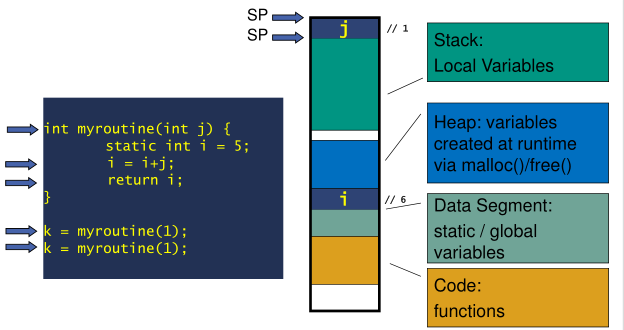
\includegraphics[scale=0.6]{running_program.png}
\caption{Laufendes C-Programm}
\end{figure}

\section{Pointer}

Etwas zu Pointern:

\begin{figure}[ht]
\centering
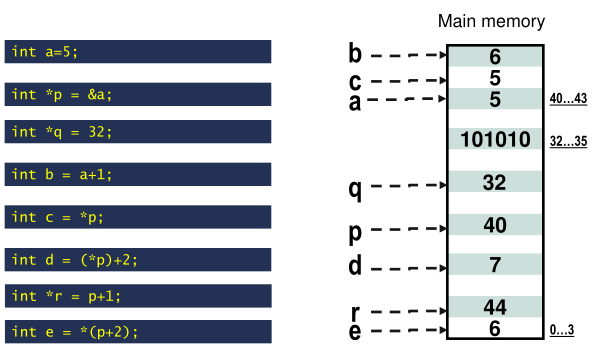
\includegraphics[scale=0.6]{pointer.png}
\caption{Pointer}
\end{figure}













\chapter{02OS}

\section{Monolithisches System}
Vorteile:
	\begin{itemize} 
		\item Einfacher Zugriff auf alle Systemdaten 
		\item Kosten von Modulinteraktionen sind niedrig
		\item Erweiterbar über Schnittstellen
		\item Vorhersehbares Verhalten 
	\end{itemize}
Nachteile:
	\begin{itemize}
		\item Kein Schutz zwischen System und Anwendung
		\item Instabil
	\end{itemize}

Beispiele:
	\begin{itemize}
		\item uCLinux, RTOSe, eCos
	\end{itemize}
	
\section{Mehrschichtiger Ansatz}
	\begin{itemize}
		\item Betriebssystem ist in n Schichten aufgeteilt
		\item Jede Schicht kann nur auf die Funktionen und Dienste von niedrigeren Schichten zugreifen 
			\begin{itemize} 
				\item Schicht 0 ist die Hardware
				\item Schicht n ist das Benutzerinterface
			\end{itemize}
		\item Einfachere Migration zwischen Plattformen
		\item Einfachere Evolution der Hardwareplattform
		\item Niedrigere Schichten implementieren Mechanismen
		\item Höhere Schichten implementieren meistens Policies
	\end{itemize}

\begin{center}
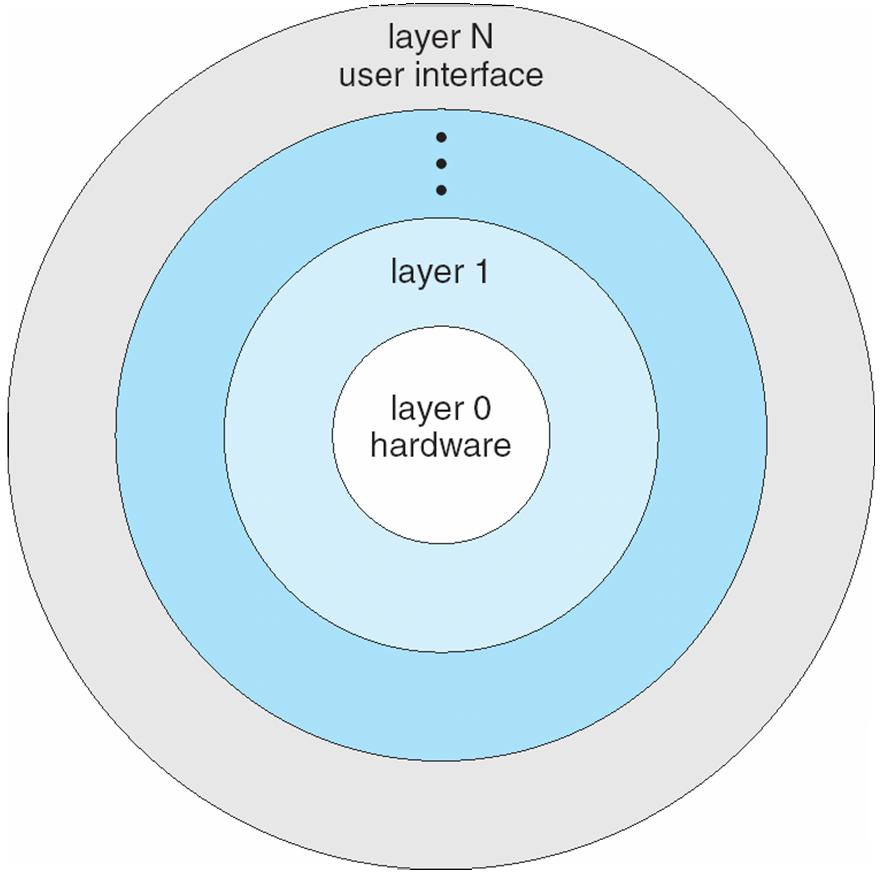
\includegraphics[scale=0.15] {schichtenmodell.png} 
\end{center}

Vorteile:
	\begin{itemize}
		\item Jede Schicht kann unabhängig getestet und verfiziert werden
		\item Korrektheit von Schicht n hängt nur von Schicht n-1 ab (einfacheres Debugging, einfachere Wartung)
	\end{itemize}

Nachteile:
	\begin{itemize}
		\item Nur unidirektionaler Schutz
		\item Beiseitige Abhängigkeit von Schichten verhindert strikte Schichtenbildung
	\end{itemize}
Beispiele:
	\begin{itemize}
		\item THE (Dijkstra), Multics(GE), VOCOS(EWSD)
	\end{itemize}
	
\section{Monolitische Kernels}
	\begin{center}
		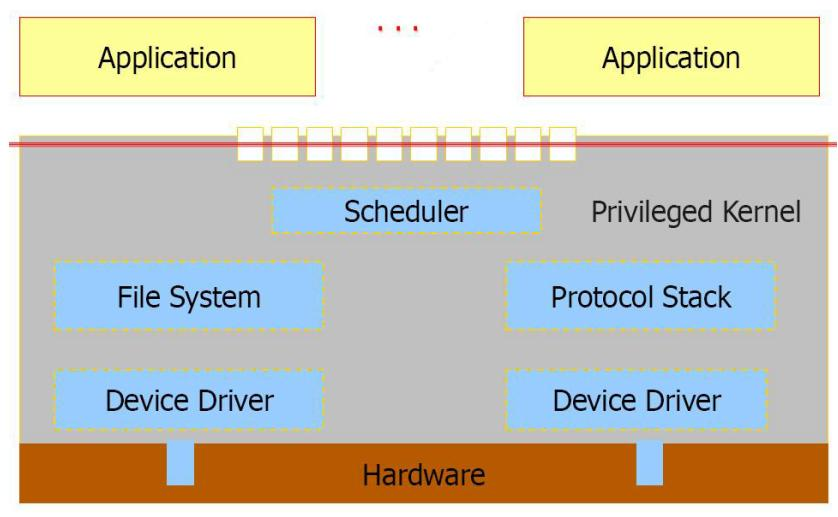
\includegraphics[scale=0.3] {monolithickernel.png}
	\end{center}
	Vorteile:
		\begin{itemize}
			\item "Gute" Performance
			\item Ausreichender Schutz zwischen Anwendungen
			\item Erweiterbar über Schnittstellen und statische/ladbare Module
		\end{itemize}
	Nachteile:
		\begin{itemize}
			\item Kein Schutz zwischen Kernel-Komponenten
			\item Nebeneffekte durch undokumentierte Interfaces
			\item Hohe Komplexität durch hohe gegenseitige Abhängigkeit
		\end{itemize}
	Beispiele
		\begin{itemize}
			\item Linux, Solaris
		\end{itemize}

\section{Microkernel Systeme}
	\begin{center}
		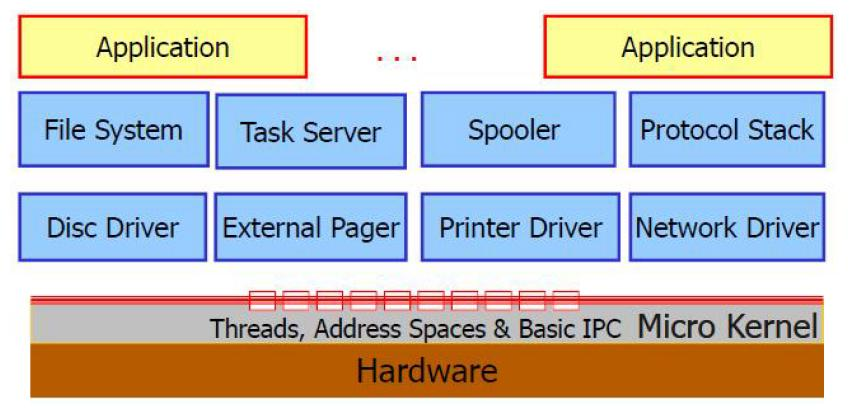
\includegraphics[scale=0.3] {microkernel.png}
	\end{center}

	\begin{itemize}
		\item Möglichst viel des Kernels in den "Benutzer" space packen
		\item Kommunikation erfolgt zwischen Benutzermodulen mit Nachrichtenweitergabe
	\end{itemize}
	
	Vorteile:
		\begin{itemize}
			\item Einfacher einen Microkernel zu erweitern
			\item Einfacher das Betriebssystem auf neue Architekturen zu portieren
			\item Zuverlässiger (es läuft weniger Code im Kernel-Modul
			\item Mehrere APIs vorhanden
			\item Verbesserte Robustheit und Sicherheit
			\item Einfacher zum Testen und Beweisen
			\item Verbesserte Wartbarkeit
		\end{itemize}
	Nachteile:
		\begin{itemize}
			\item Performance Unkosten durch Kommunikation von Benutzerspace zum Kernelspace 
			\item Zusätzliche Zersetzung
			\item Schlechte Erfahrungen mit IBMs Workplace OS (1991-1995)
		\end{itemize}

\section{Virtuelle Maschinen}
	\begin{itemize}
		\item Eine virtuelle Maschine nimmt den mehrschichtigen Ansatz und behandelt Hardware sowie den Kernel des Betriebssystems so als wären sie Hardware
		\item Eine virtuelle Maschine stellt ein identisches Interface zu der blanken, darunterliegenden Hardware
		\item Der Betriebssystem-Host kreiert die Illusion das ein Prozess sein eigenen Prozessor und (virtuellen Speicher) hat.
		\item Jeder Gast bekommt eine Kopie des darunterliegenden Computers zur Verfügung gestellt.
	\end{itemize}
	Vorteile:
		\begin{itemize}
			\item Mehrere Betriebssysteme können sich die gleiche Hardware teilen
			\item Gegenseitiger Schutz
			\item Nützlich für Development und Testen
		\end{itemize}
	\begin{center}
		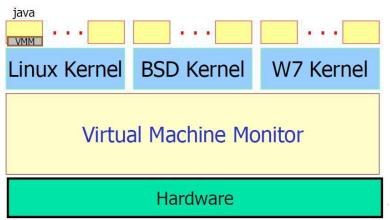
\includegraphics[scale=0.5] {virtualmachine.png}
		\\
		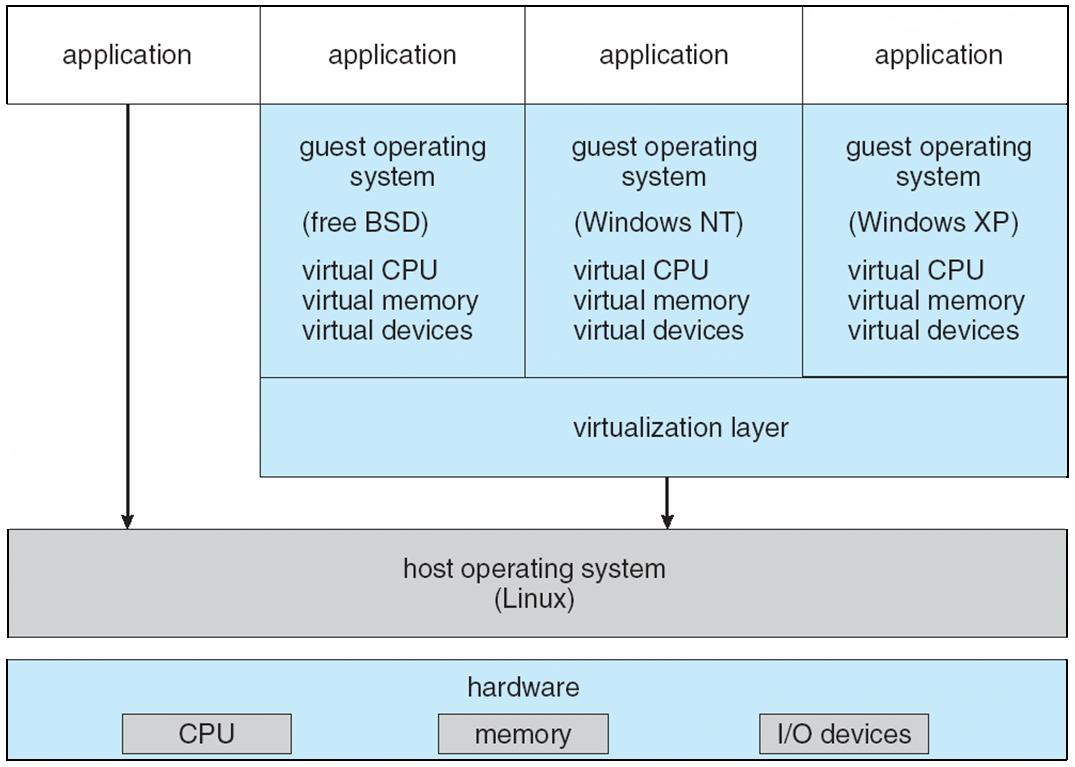
\includegraphics[scale=0.35] {vmwarearchi.png}
		\\
		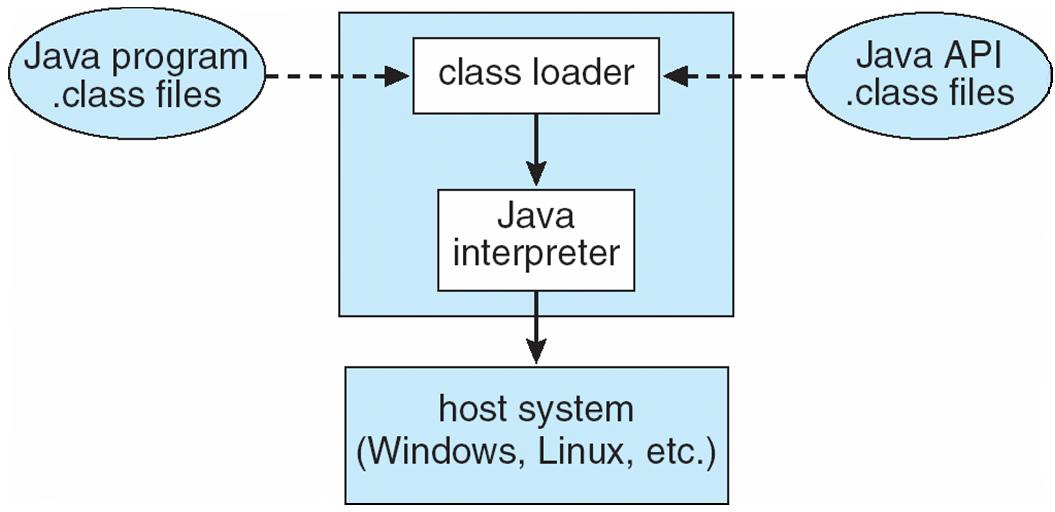
\includegraphics[scale=0.3] {javavm.png}
	\end{center}


\chapter{03aProcess-management}

\section{Konzept}
	Ein Betriebssystem führt
	\begin{itemize}
		\item Batch System - Jobs
		\item und Zeitteilende Systeme - Benutzerprogramme oder -aufgaben
	\end{itemize} 
	aus.\\
	Job oder Prozess := ein Programm in Ausführung
\section{Process Structure (in memory)}
	\begin{figure}[htbp]
		\begin{minipage}[t]{10cm}
			\vspace{0pt}
			Ein Prozess beinhaltet
			\begin{itemize}
				\item einen Programmzähler
				\item Register
				\item den Code
				\item einen Stack
				\item Daten
				\begin{itemize}
					\item Rodata: lesen (read-only)
					\item Data: lesen und schreiben
					\item BSS: globale, statische Variablen auf 0 gesetzt
				\end{itemize}
				\item eine Heap
			\end{itemize}
		\end{minipage}
		\hfill
		\begin{minipage}[t]{4cm}
			\vspace{0pt}
			\centering
			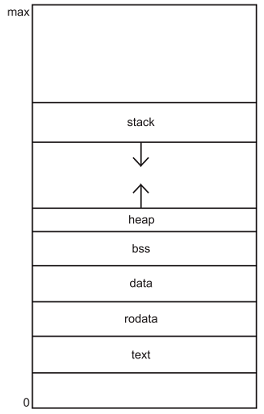
\includegraphics[scale = 0.3]{memory.png}\\
		\end{minipage}
	\end{figure}

\section{Process Status}
	Ein Prozess wechselt wie folgt zwischen verschiedenen Zuständen:\\ \\
	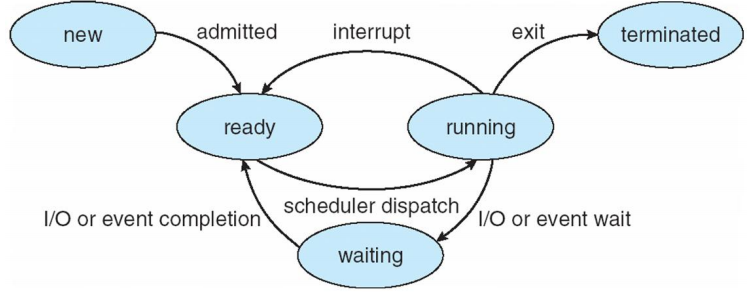
\includegraphics[scale = 0.4]{prozess_status.png}
\section{Process Control Block(PCB)}
	Zu jedem Prozess gehört:
	\begin{itemize}
		\item ein Prozessstatus und eine ID
		\item ein Programmzähler
		\item CPU - Register
		\item CPU - Scheduling Informationen
		\item Berechtigungen
		\item Ein- und Ausgabe Informationen
	\end{itemize}
\section{Context Switch}
	:= Das Wechseln der Prozessinformationen beim Prozesswechsel in der CPU\\ \\
	Dieser Kontext wird in PCB's gespeichert. Zeit zum Wechseln geht bei der Rechenzeit verloren.\\ \\
	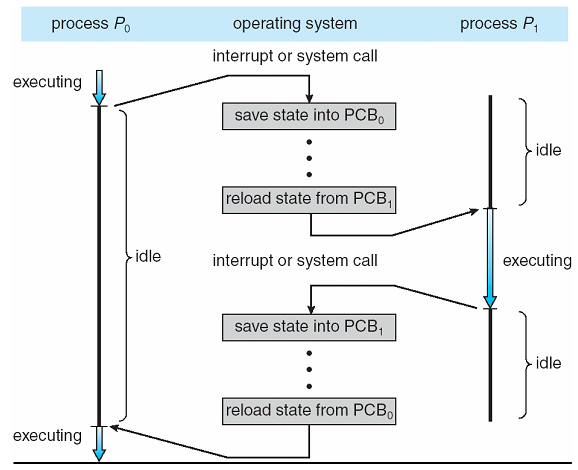
\includegraphics[scale = 0.6]{process_switch.png}\\
\section{Process Creation}
	\begin{itemize}
		\item Prozesse bilden als Kinder- und Elternprozesse einen Prozessbaum
		\item Prozesse werden durch einen Process Identifier (pid) erkannt und verwaltet
		\item Resource Sharing
		\begin{itemize}
			\item Kinder und Eltern teilen \textbf{alle} Resourcen
			\item Eltern teilen einen Teil ihrer Resourcen mit ihren Kindern
			\item Kinder und Eltern teilen \textbf{keine} Resourcen
		\end{itemize}
		\item Synchornisation
		\begin{itemize}
			\item Eltern und Kinder werden zeitgleich ausgeführt
			\item Eltern warten auf die Terminierung der Kinder
		\end{itemize}
		\item Adressraum
		\begin{itemize}
			\item Kind kopiert den Adressraum
			\item Kind lädt ein Programm
		\end{itemize}
		\item UNIX Beispiele
		\begin{itemize}
			\item \underline{fork} SysCall erzeugt neuen Prozess
			\item \underline{exec} SysCall benutzt nach \underline{fork} um neues Programm zu laden
		\end{itemize}
	\end{itemize}
	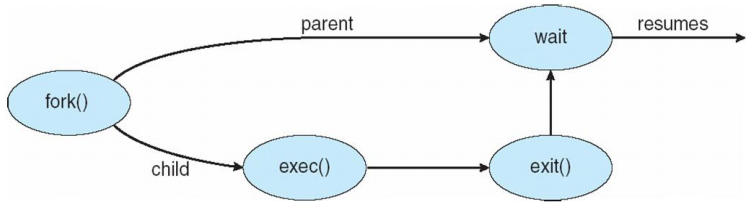
\includegraphics[scale = 0.6]{process_fork.png}
\chapter{03bProcess-management-scheduling}
\chapter{04Process-coordination}

\section{Interprozess Kommunikation}
	\begin{itemize}
		\item Prozesse in einem System können unabhängig oder zusammenarbeitend sein
		\item Zusammenarbeitende Prozesse können sich andere oder von anderen Prozessen beeinflusst werden
		\item Zusammenarbeitende Prozesse benötigen interprocess communication (IPC -> 2 Modelle: Shared memory, message passing)
	\end{itemize}
	Gründe für zusammenarbeitende Prozesse:
	\begin{itemize}
		\item Schnellere Berechnung
		\item Komfort/Einfachheit
		\item Modularität
		\item Teilen von Informationen
	\end{itemize}

\subsection{Nachrichtenweitergabe (Message Passing)}
	\begin{itemize}
		\item Mechanismus für Prozesse um zu kommunizieren und ihre Aktionen zu synchronisieren
		\item IPC-Einrichtung bietet zwei Operationen: receive, send (Nachrichtengröße ist fix oder variabel)
	\end{itemize}
\subsubsection {Direkte Kommunikation}
	\begin{itemize}
		\item Prozesse müssen sich gegenseitig explizit per Namen nennen
		\item send(P, Nachricht) - schicke eine Nachricht an Prozess P
	\end{itemize}
	Eigenschaften:
	\begin{itemize}
		\item Links werden automatisch eingerichtet
		\item Ein Link wird genau mit einem Paar von kommunizierenden Prozessen assoziiert
		\item Jedes Paar besitzt genau einen Link
		\item Ein Link könnte unidirektional sein, ist aber meistens bi-direktional
	\end{itemize}
	
\subsubsection{Indirekte Kommunikation}
	\begin{itemize}
		\item Nachrichten werden von Mailboxes (ports) gelenkt und empfangen
		\item Jede Mailbox hat eine einzigartige ID
		\item Prozesse können nur kommunizieren wenn sie eine Mailbox teilen
	\end{itemize}
	Eigenschaften:
	\begin{itemize}
		\item Ein Link wird nur eingerichtet falls Prozssse eine Mailbox teilen
		\item Ein Link kann mit vielen Prozessen assoziiert werden
		\item Jedes Paar von Prozessen kann mehere Kommunikationslinks teilen
		\item Links können unidirektional oder bi-direktional sein
	\end{itemize}
	Operationen:
	\begin{itemize}
		\item Neue Mailbox erstellen
		\item schicken und empfangen von Nachrichten über die Mailbox
		\item Mailbox löschen
	\end{itemize}
	
\section{Synchronisation}
	\subsection {Producer-Consumer Problem}
		\begin{itemize}
			\item Problemstellung der Prozesssynchronisation die eine Regelung der Zugriffsreihenfolge auf einer Datenstruktur von Prozessen bzw Thread thematisiert
			\item Prozesse sind Erzeuger oder Verbraucher
		\end{itemize}	
	\subsubsection{Critical-Section-Problem}
		\begin{itemize}
			\item Mutual Exclusion: Wenn Prozess P in seinem kritischen Bereich ist, kann kein anderer Prozess in seinen kritischen Bereich
			\item Progress:  Wenn kein Prozess in seinem kritischen Bereich ausgeführt wird, aber mehrere Prozesse den kritischen Bereich betreten möchten, kann die Auswahl der Prozesse die als nächstes eintreten nicht unbegrenzt aufgeschoben werden
			\item Bounded Waiting: Es muss eine zeitliche Grenze existieren, sodass Prozesse nicht verhungern. (z.B. Prozess A,B wechseln sich in im kritischen Bereich ab obwohl Prozess C auch den kritischen Bereich betreten möchte, Prozess C verhungert)
			\item Viele Systeme bieten Hardwaresupport für critical section code
		\end{itemize}
	\subsection{Semaphore}
		\begin{itemize}
			\item Synchronisationstool das kein "busy waiting" benötigt
			\item Weniger kompliziert
			\item Nur zwei Standardoperationen für die Modifikation eines Semaphores erlaubt: wait(), signal()
			\item Counting semaphore - integer Wert unbegrenzt
			\item Binary semaphore - integer Wert kann zwischen 0 und 1 variieren 
		\end{itemize}

\section{Deadlock and Starvation}
		\begin{itemize}
			\item Deadlock - zwei oder mehr Prozesse warten unbegrenzt auf eine Aktion die nur von einem wartenden Prozess ausgeführt werden kann
			\item Starvation - Ein Prozess könnte nie von einer Semaphorewarteschlange entfernt werden
			\item Priority Inversion - Scheduling-Problem, wenn ein Prozess niedriger Priorität einen Platz hält den ein Prozess höherer Priorität braucht
		\end{itemize}
		
\section{Klassische Probleme der Synchronisation}
		\begin{itemize}
			\item Bounded-Buffer Problem
			\item (First-, Second-, Third-) Readers und Writers Problem
			\item Philosophenproblem
			\item Weitere Probleme: "The Art for Multiprocessor Programming"
		\end{itemize}
		
	\subsection{Bounded-Buffer Problem}
		\begin{itemize}
			\item N Buffer, jeder kann ein Item halten. Init:
				\begin{itemize}
					\item Semaphore mutex = 1
					\item Semaphore full = 0
					\item Semaphore emptry = N
				\end{itemize}
		\end{itemize}
	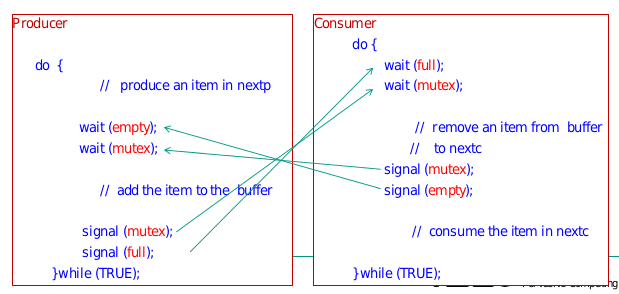
\includegraphics[scale=0.75] {boundedbufferprob.png}
	
	\subsection{Readers-Writers Probleme}
		\begin{itemize}
			\item Ein Datenset wird zwischen einer Anzahl nebenläufiger Prozesse geteilt
			\begin{itemize}
				\item Readers - Können nur das Datenset lesen (führen KEINE Updates durch)
				\item Writers - Können das Datenset lesen und beschreiben
			\end{itemize}
			\item Problem - erlaube mehreren Readers zur gleichen Zeit zu lesen. Lediglich ein Writer kann auf die shared data zur gleichen Zeit zugreifen
		\end{itemize}
			
			\subsubsection{First-Readers-Writers Problem}
				\begin{itemize}
					\item Kein Reader sollte warten wenn ein shared date gelesen werden kann
				\end{itemize}	
			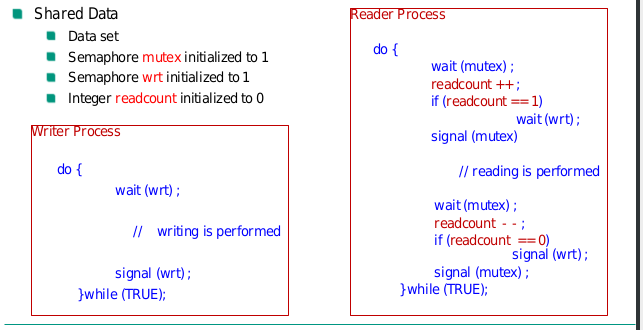
\includegraphics[scale=0.6] {readerwriterprob.png}
			
			\subsubsection{2nd und 3rd Readers-Writers Problem}
				\begin{itemize}
					\item 2nd Readers-Writers Problem: Kein Writer, der einmal einer Warteschlange hinzugefügt wurde, sollte nicht länger als absolut nötig warten
					\item 3rd Readers-Writers Problem: Keinem Thread sollte es erlaubt sein zu verhungern (starve)
				\end{itemize}
		\subsection{Philosophenproblem}
			\begin{itemize}
				\item 5 Philosophen
				\item Zyklischer Ablauf
				\item => Deadlock
			\end{itemize}
			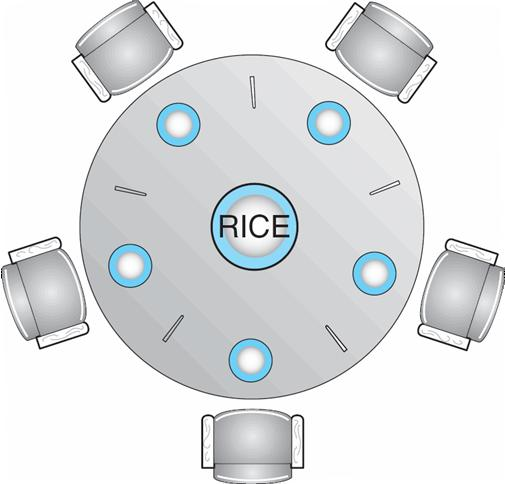
\includegraphics[scale=0.35] {philprob.png}
	\section{Deadlocks}
		\subsection{Das Deadlock Problem}
			\begin{itemize}
				\item Ein Set von geblockten Prozessen die eine Ressource halten und auf eine andere Ressource die von einem anderen Prozess gehalten wird warten
				\item Beispiel: P1 und P2 halten jeweils ein disk drive, benötigen und warten auf das das jeweils andere
			\end{itemize}
		\subsection{System Model}
			\begin{itemize}
				\item Ressourcentypen: R1, R2, ..., Rm (CPU Zyklen, Speicherplatz, I/O Geräte)
				\item Jeder Ressourcen Typ Ri hat Wi Instanzen
				\item Jeder Prozess verwendet eine Ressource mit: "request", "use" und "release"
			\end{itemize}
		\subsection{Deadlock Charakterisierung}
			\begin{itemize}
				\item Mutual exclusion: Zu einer Zeit kann nur ein Prozess eine Ressource benutzen
				\item Hold and wait: Ein Prozess hält mindestiens eine Ressource und wartet auf zusätzliche Ressource die von anderen Prozesse gehalten werden
				\item No preemption: Eine Ressource kann nur freiwillig von einem Prozess der sie hält, nachdem der Prozess seine Aufgabe beendet hat, freigegeben werden
				\item Circular wait: Set von wartenden Prozesse (P0, P1, ..., P1) und P0 wartet auf eine Ressource die P1 hält, P1 auf eine Ressource die P2 hält, ..., Pn wartet auf eine Ressource die P0 hält
			\end{itemize}
		\subsection{Resource-Allocation Graph}
			\begin{itemize}
				\item request edge - Kante von P1 nach Rj
				\item assignment edge - Kante von Rj nach Pi
			\end{itemize}
		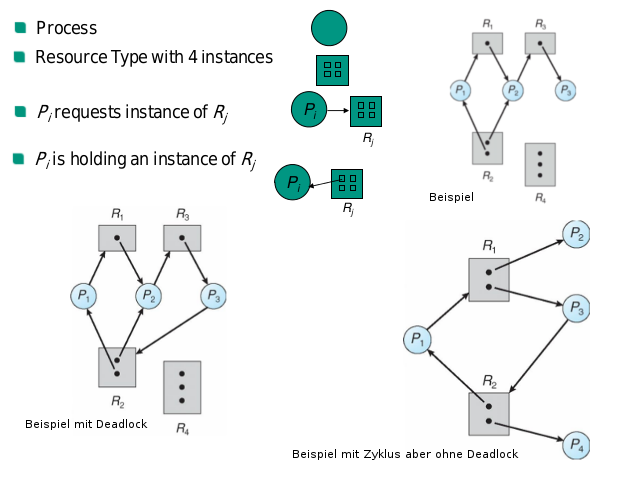
\includegraphics[scale=0.7]{resallograph.png}
			\begin{itemize}
				\item Graph beinhaltet kein Zyklus => kein Deadlock
				\item Graph beinhaltet Zyklus =>
					\begin{itemize}
						\item Falls jeweils nur eine Instanz pro Ressource, Deadlock
						\item Falls mehrere Instanzen pro Ressource, Deadlock möglich
					\end{itemize}
			\end{itemize}
		\subsection{Methoden für Handling Deadlocks}
			\begin{itemize}
				\item Sicherstellen das, dass System nie in einen Deadlockzustand eintritt
				\item Dem System den Eintritt in einen Deadlockzustand erlauben und dann recovern
				\item Problem ignorieren und annehmen das Deadlocks nie auftreten (wird von den meisten Betriebssystemen verwendet)
			\end{itemize}
		\subsection{Deadlock Vorbeugung}
			\begin{itemize}
				\item Mutual Exclusion: wird nicht für teilbare Ressource benötigt; muss gehalten werden für nicht teilbare Ressourcen
				\item Hold and Wait: musst garantieren das jederzeit wenn ein Prozess eine Ressource anfrägt, der Prozess selbst keine anderen Ressourcen hält
				\item No Preemption: 
					\begin{itemize}
						\item Wenn ein Prozess einige Ressource hält und eine andere anfrägt und diese nicht gleich bekommt, dann werden alle Ressource die gerade gehalten werden freigegeben
						\item Preempted Ressourcen werden zu einer Liste von Ressourcen hinzugefügt für welche der Prozess wartet
						\item Prozess restartet nur wenn er seine alten Ressourcen sowie die neue bekommt
					\end{itemize}
				\item Circular Wait: Führe eine totale Ordnung von allen Ressourcentypen ein und veranlasse das jeder Prozess Ressourcen in einer aufsteigenden Ordnung von Aufzählungen anfrägt
			\end{itemize}
		
		\subsection {Deadlock Vermeidung}
			\begin{itemize}
				\item Das einfachste und nützlichste Modell benötigt das jeder Prozess ein Maximum an Ressourcen von jedem Typ die er benötigt deklariert
				\item Der deadlock-avoidance Algorithmus untersucht den resource-allocation Zustand, um sicherzustellen das es nie eine circular-wait condition gibt
				\item Resource-allocation state ist durch die Anzahl der verfügbaren und alloziierten Ressourcen und den maximal Zugriffen auf Prozesse definiert 
			\end{itemize}
			
			\subsubsection{Safe State}
				\begin{itemize}
					\item Wenn ein Prozess eine verfügbare Ressource anfrägt, muss das System sicherstellen das die unmittelbare Allokation das System in einem safe state lääst
					\item Ein System ist in einem safe state, wenn eine Sequenz <P1, P2, ..., Pn> von allen Prozessen existiert und das System für jeden Prozess Pi die Ressourcen die Pi anfragen kann gerade verfügbar sind. (and resources held by all the Pj with j < l)
				\end{itemize}
				\begin{itemize}
					\item System ist in safe state => keine Deadlocks
					\item System ist in unsafe state => Deadlocks möglich
					\item Vermeidung => sicherstellen das ein System nie in einen unsafe state eintreten kann
				\end{itemize}
				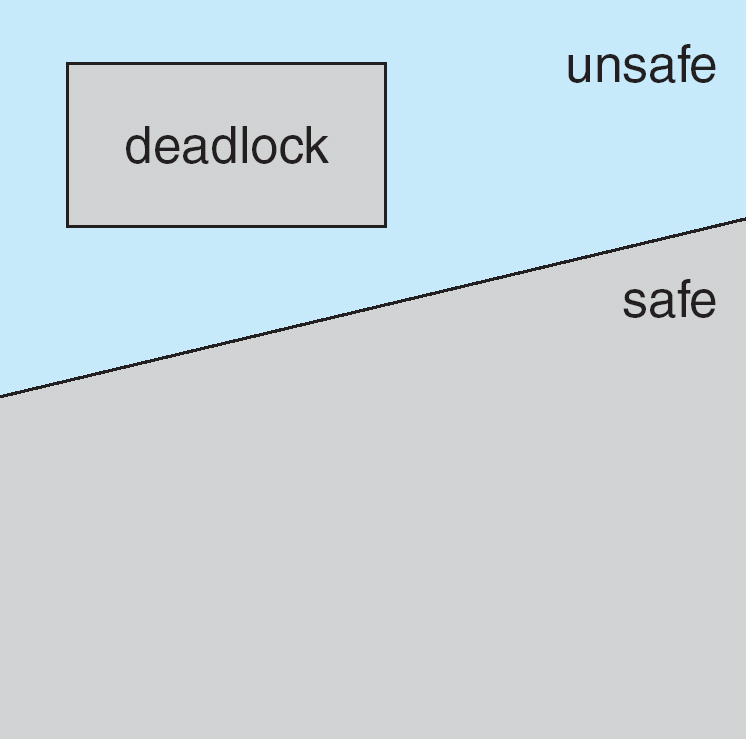
\includegraphics[scale=0.15] {state.png}
			
			\subsubsection{Vermeidungsalgorithmen}
				\begin{itemize}
					\item Eine Instanz von jedem Ressourcentyp => resource-allocation graph benutzen
					\item Mehr Instanzen von jeden Ressourcentyp => banker's Algorithmus
				\end{itemize}
	\subsection{Recovery from Deadlock}
				\begin{itemize}
					\item Process Termination
						\begin{itemize}
							\item Abbruch aller deadlocked Prozesse
							\item Prozess nach Prozess wird abgebrochen bis der Deadlockzyklus eliminiert wurde
						\end{itemize}
					\item Resource Preemption
						\begin{itemize}
							\item Wähle ein "Opfer" - minimieren kosten
							\item Wiederherstellung - zu einem safe state zurückkehren, die Prozesse für den Zustand neustarten
							\item Starvation - Gleicher Prozess könnt immer als Opfer ausgewählt werden, Anzahl der Wiederherstellungen im Kostenfaktor berücksichtigen
						\end{itemize}
				\end{itemize}

\chapter{05aMemoryManagement}
\section{Background}
\begin{itemize}
\item Damit ein Programm laufen kann muss es von der Platte in den Speicher gebracht und innerhalb des Prozesses plaziert werden.

\item Auf Hauptspeicher und Register kann nur die CPU direkt zugreifen.

\item Ein Register Zugriff beträgt einen CPU Takt (oder weniger)

\item Hauptspeicher kann einige Zyklen dauern.

\item Cache liegt zwischen Hauptspeicher und CPU Registern

\item Sicherheit des Speichers werden zur Sicherstellung korrek ausgeführter Operationen benötigt.

\end{itemize}

\subsection{Speicherpartitionierung}

Hauptspeicher wird normalerweise in zwei Partitionen unterteilt :
\begin{description}
\item[Resident operating system]\ \\ werden normalerweise im "`low memory"' mit  \textit{interrupt vector} gespeichert
\item[User processes]\ \\werden im "`high memory"' gespeichert
\end{description}

Register dienten dem Schutz der Benutzerprozesse untereinander und vor Veränderungen von Betriebssystemcode und Daten.
\begin{itemize}
\item "`Base register"' beinhalten den Wert der kleinsten physichen Adresse.
\item "`Limit register"' beinhalten den Umfang der logischen Adressen.
\end{itemize}

\begin{center}
		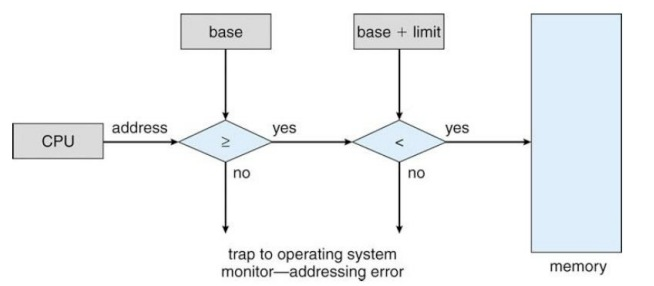
\includegraphics[scale=0.5] {baseandlimit.png}
\end{center}

\subsection{Einfacher Schutz mit \textit{base} und \textit{limit register}}

Ein Paar aus base und limit Registern definieren einen logischen Adressraum

\begin{center}
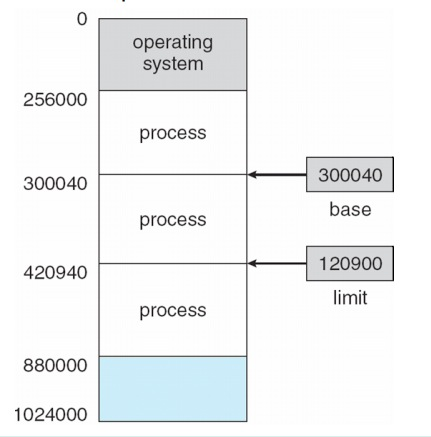
\includegraphics[scale=0.5]{baseandlimitprotection.png}
\end{center}


\section{Swapping}
\begin{itemize}
\item Ein Prozess kann temporär aus dem Speicher in einen Zusatzspeicher gewechselt werden und dann wieder zurück um die Ausführung fortzusetzen
\item \textbf{Zusatzspeicher (\textit{Backing store})} \ \\ Schneller Speicher, welcher groß genug ist um alle \textit{memory images} aller Nutzer unterzubringen. Er muss jedoch direkten Zugriff zu jenen bieten.
\item \textbf{Roll out, roll in} \ \\ Eine Swapping Variation für prioritätsbasierte scheduling Algorithmen: Prozesse niedriger Priorität werden mit Prozessen hoher Priorität ausgewechselt um somit geladen und ausgeführt werden können.
\item Hauptbestandteil der \textit{swap time} ist die \textit{transfer time}: Die totale Transferzeit ist direkt proportional zur Menge des ausgewechelten Speichers
\item Modifizierte Versionen von ˆ\textit{swapping} wird auf vielen System gefunden (z.B UNIX, Linux und Windows)
\item Das System führt eine \textit{ready queue} mit "`ready to run"'-Prozessen welche ein memory image im Speicher haben.

\end{itemize}

\begin{figure}[ht]
\centering
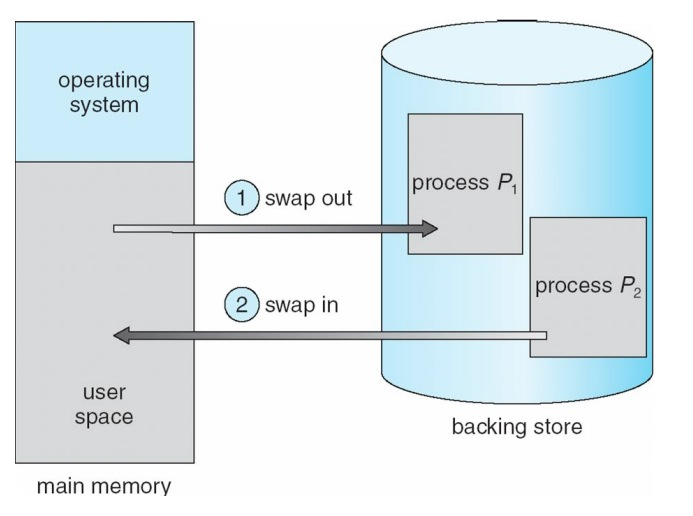
\includegraphics[scale=0.6]{swapping.png}
\caption{Schematik von Swapping}
\end{figure}

\section{Allocation}
\subsection{Zusammenhängende Allokierung (\textit{contiguous allocation)}}
\subsubsection{Multiple Partitions Allokierung}
\begin{itemize}
\item \textit{Hole}: Blöcke an verfügbarem Speicher. Löcher verschiedener Größe sind über den ganzen Speicher verteilt
\item Bei Ankunft eines Prozesses, wird Speicher von einem Loch, welches groß genug ist um den Prozess aufzufassen, allokiert
\end{itemize} Das Betriebssystem kümmert sich um Informationen über:

\begin{itemize}
\item[a)] allokierte Partitionen
\item[b)] freie Partitionen (Löcher)
\end{itemize}

\begin{figure}[ht]
\centering
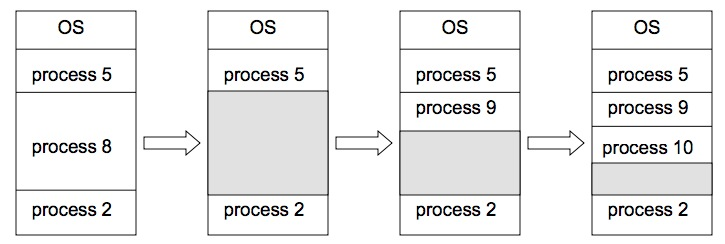
\includegraphics[scale=0.6]{allocation.png}
\caption{Schematik Speicherallokierung}
\end{figure}

\subsection{Dynamisches Speicher-Allokations Problem}
\textbf{Problem:} Wie befreidigt man Anfragen der Größe n von einer Liste mit freien Löchern?
\begin{itemize}
\item \textit{First-fit}: Allokiert das erste Loch, welches groß genug ist: schnellste Allokierungsstrategie, hinterlässt jedoch Löcher unterschiedlicher Größe
\item \textit{Best-fit}: Allokiert das kleinste passende Loch. Es muss jedoch die komplette Liste durchsucht werden, außer sie ist nach Größe sortiert. Hinterlässt die kleinsten Löcher.
\item \textit{Worst-fit}: Allokiert das größte Loch. Es muss die gesammte Liste durchsucht werden, hinterlässt die größten Löcher
\item \textit{Next-fit}: Nächst passendes Loch nach der letzten Allokierung
\item \textit{Buddy System}:
\begin{itemize}
\item Die Löcher werden in k Listen so einsortiert, dass die i-te Liste jeweils Löcher der Länge gleich $2^i/$ für i = 1,...,k enthält
\item Dabei können zwei benachbarte Löcher der i-ten Liste effizient zu einem  Loch der i+1-ten Liste zusammengefügt werden
\item Umgekehrt kann ein Loch der i-ten Liste einfach in zwei Löcher der i-1-ten Listen aufgeteilt werden
\item Löcher im Buddy-System können effizient mittels eines Binärbaumes dargestellt werden
\item Laufzeitverhalten: Zuweisen und Freigabe Block schneller als first/best-fit. Fragmentierungsbehandlung ist aufwändiger. Deshalb Lazy-\textbf{Buddy:Zusammenfügen "`selten"'}
\item Standard für Unix/Linux
\end{itemize}
\end{itemize}

\begin{figure}[ht]
\centering
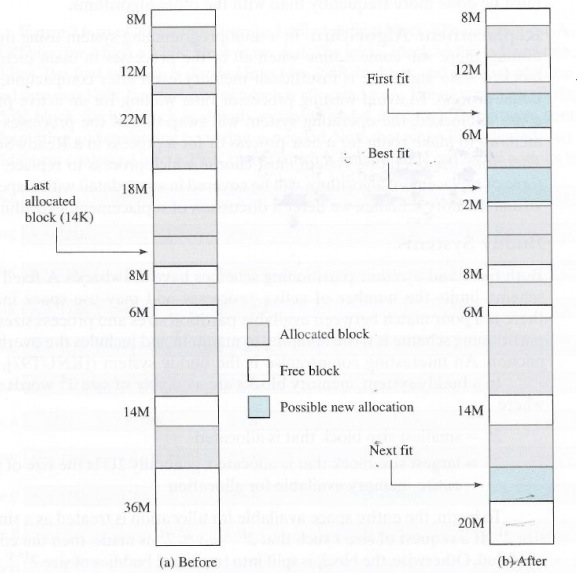
\includegraphics[scale=0.55]{allocationexample.png}
\caption{Beispiel vor und nach Allokierung eines 16Mbyte Blocks}
\end{figure}

\begin{figure}[ht]
\centering
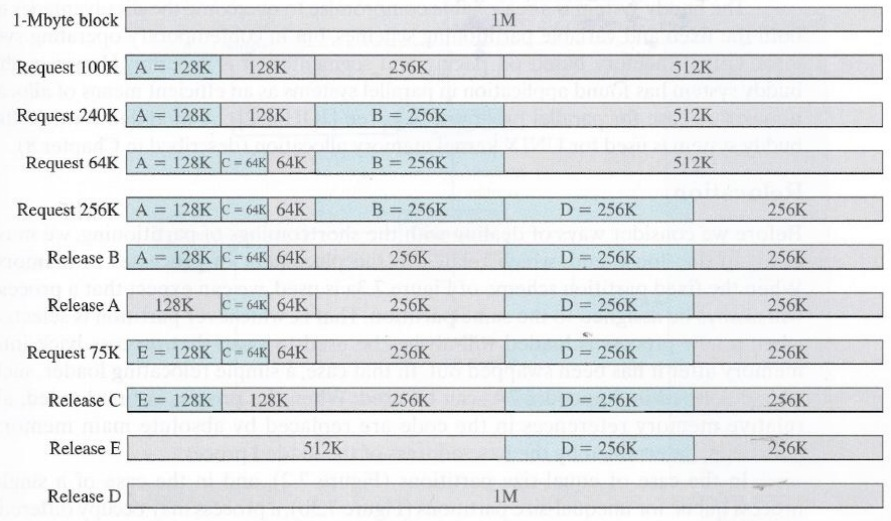
\includegraphics[scale=0.50]{buddysystem.png}
\caption{Beispiel Buddysystem}
\end{figure}
  \ \\
\begin{figure}[ht]
\centering
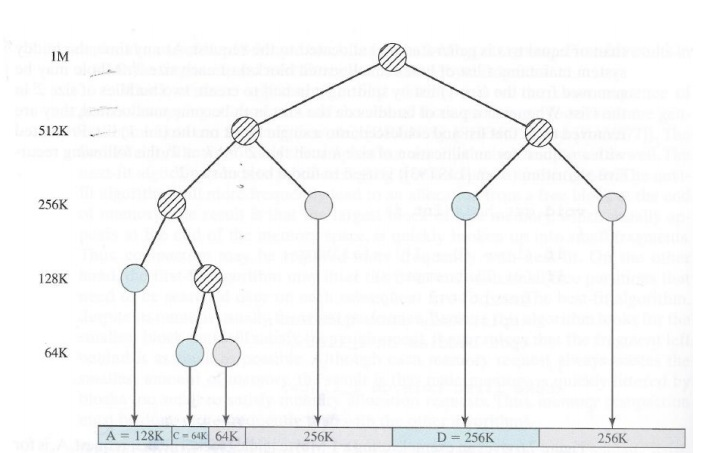
\includegraphics[scale=0.5]{buddysystemtree.png}
\caption{Darstellung Buddysystem als Baum}
\end{figure}
\newpage

\section{Relocation}
\subsection{Fragmentierung}
\begin{itemize}
\item \textbf{Externe Fragmentierung} - Es ist genügend Speicher vorhanden um eine Anfrage zu befriedigen, jedoch nicht zusammenhängend.
\item \textbf{Interne Fragmentierung} - Allokierter Speicher kann ein wenige größer als der angeforderte Speicher sein: Der Größenunterschied ist Speicherintern innerhalb einer Partition, wird jedoch nicht verwendet
\item Reduzierung externer Fragmentierung durch Verdichtung (\textit{compatction}):
\begin{itemize}
\item Vermische den Speicherinhalt um alle freien Speicher in einem großen Block zu sammeln
\item \textit{Compaction} ist nur dann möglich wenn die \textit{relocation} dynamisch und während der Durchführungszeit statt findet

\end{itemize}
\end{itemize}
\subsection{Adressabbildung und "`Data to Memory"'}

\begin{itemize}
\item \textbf{Compile time}: Wenn der Speicherstelle  a priori bekannt ist, kann ein absoluter Code generiert werden. Muss jedoch recompiliert werden wenn der Startpunkt verändert wir.
\item \textbf{Load time}: Muss versetzbaren (engl.: \textit{relocatable}) Code generieren wenn die Speicherstelle zur Übersetzungszeit nicht bekannt ist.
\item \textbf{Execution time}: Verzögerung der Abbildung während der Laufzeit, wenn der der Prozess während der Ausführung von einem Speichersegment zu einem anderen bewegt werden kann. 
\end{itemize}

\subsection{Logische vs. Physicher Adressraum}

\begin{itemize}
\item \textbf{logische Adresse} - CPU generiert, auch als virtuelle Adresse bezeichnet
\item \textbf{physische Adresse} - von der Speichereinheit gesehene Adresse.

Logische und physische Adressen sind im Sinne von Kompilierzeit und "`load-time adress-binding-schemes"' gleich. Unterschied liegt in der "`execution-time adress-binding scheme"'
\end{itemize}

\subsection{Memory-Management Unit (MMU)}
\begin{itemize}
\item Hardware Geräte welche virtuellen auf physikalischen Adressen abbilden
\item Auf jede Adresse, die von einem Nutzerprozess generiert wurde, wird der Wert der relocation register addiert um die Hardwareadresse zu ermitteln.
\item Das Endnutzerprogramm setzt sich mit den logischen Adressen auseinander, nie mit den real physischen.
\end{itemize}

\subsection{Dynamic Loading}
\begin{itemize}
\item Routine wird nicht geladen bis es aufgerufen wird
\item Routine wird auf der Platte in einem verlagerbaren Zustand format behalten
\item Nützlich wenn große  Mengen an Code unregeläßig auftretende Fälle behandelt werden müssen
\item Es wird keine besondere Unterstützung durch das Betriebssystem benötigt: Service wird vom "`relocatable linking loader"' bereitgestellt
\item Bessere Nutzung von Speicherraum
\begin{itemize}
\item Ungenutzte Routinen werden nie geladen
\item Überlagerung macht das Laden von Modulen für die momentane Ausführungsphase möglich \begin{tiny}
(the hell does that mean?)
\end{tiny}
\end{itemize}
\end{itemize}

\begin{figure}[ht]
\centering
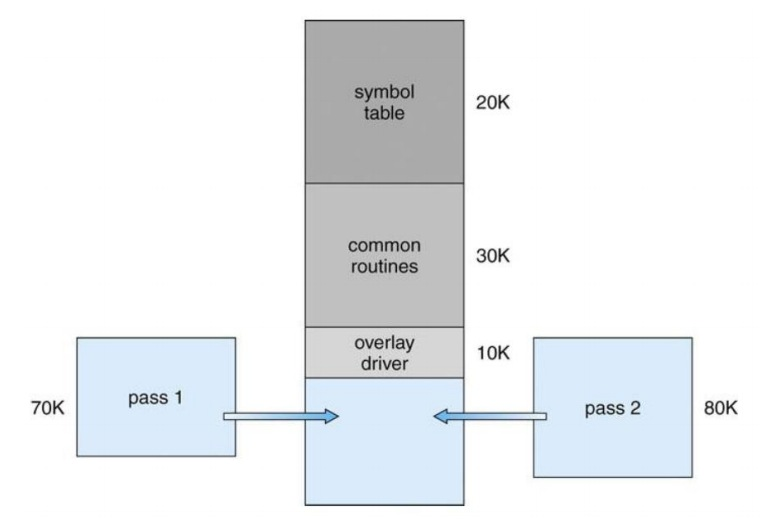
\includegraphics[scale=0.50]{overlays.png}
\caption{Überlagerung (\textit{overlays})}
\end{figure}

\subsection{Dynamic Linking (Share Libraries)}
\begin{itemize}
\item Routine wird nicht gelinked bis es aufgerufen wird (linking wird aufgeschoben (engl.: \textit{postponed}))
\item Kleinere Teile an Code, sogenannte Stubs, dienen dazu die angemessene "`memory-resident library routine"' festzustellen (oder wie man die routine library lädt)
\item Stub ersetzt sich selbst mit der Adresse der Routine und führt es dann aus
\item Betriebssystem muss checken ob sich die Routine  bereits im Speicherraum anderer Prozesse befindet
\item Dynamisches Linken ist vorallem für die Updates von Libraries stützend.
\end{itemize}

\section{Segmentation}
\begin{itemize}
\item Speicherverwaltungs Schema, welches Nutzeransicht des Speichers fördert.
\item Ein Proramm ist eine Sammlung an Segmenten. Segmente sind z.B
\begin{itemize}
\item \textit{main program}
\item \textit{procedure}
\item \textit{function}
\item \textit{method}
\item \textit{object}
\item \textit{local/global variables}
\item \textit{common block}
\item \textit{stack}
\item \textit{symbol table}
\item \textit{arrays}

\end{itemize}
\end{itemize}
\subsection{Architektur}
\begin{itemize}
\item Logische Adresse besteht aus einem Tupel:
\begin{itemize}
\item <segment-nummer, offset>
\item offset = Abstand (\textit{displacement (d)})
\end{itemize}

\item \textbf{Segment table} : Bildet zwei-dimensionale physikalische Adressen ab. Bestehen aus
\begin{itemize}
\item \textbf{base} - behinaltet die physikalische Startadresse wo sich das Segment im Speicher befindet.
\item \textbf{limit} - spezifiziert die Länge des Segments
\end{itemize}

\item \textbf{Segment-table base register (STBR)}: Zeigt auf die Stelle des Segment Tables im Speicher

\item \textbf{Segment-table length register (STLR)}: Zeigt die Anzahl vom Programm genutzten Segmente an. Diese Nummer s ist gültig wenn s < STLR

\item Protection
\begin{itemize}
\item Mit jedem Eintrag im Segment Table in Verbindung gebracht:
\begin{itemize}
\item Validierungs bit = 0 => Illegales Segment
\item Lese/Schreib/Ausführungs Rechte
\end{itemize}
\end{itemize}

 \item Protection bits mit Segmenten in Verbindung gebracht, da "`code sharing"' auf Segment Level auftritt
 
 \item Da sich Segmente in ihrer Größe unterscheiden ist die Speicherallokierung ein "`dynamic storage-allocation" Problem
 
 \begin{figure}[ht]
\centering
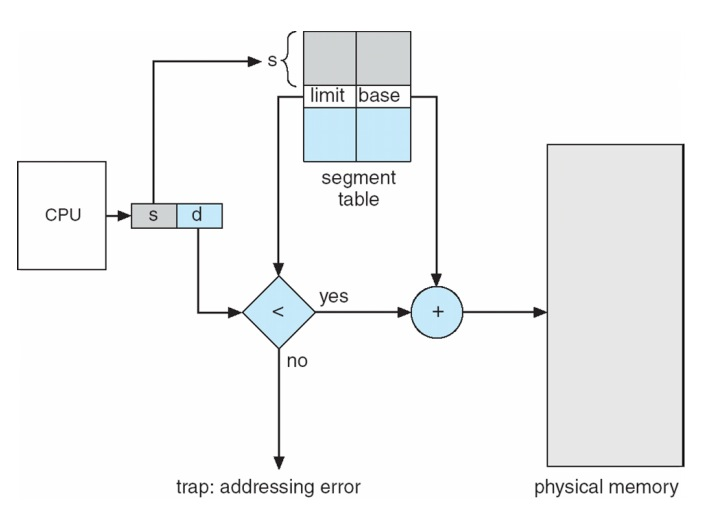
\includegraphics[scale=0.50]{segmentierung1.png}
\caption{Segmentierung Beispiel}
\end{figure}

\begin{figure}[ht]
\centering
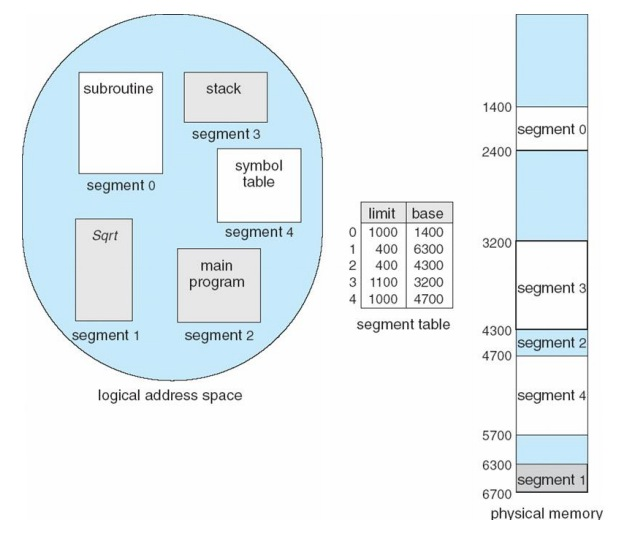
\includegraphics[scale=0.50]{segmentierung2.png}
\caption{Segmentierung Beispiel 2}
\end{figure}
\end{itemize}


\newpage
\section{Paging}
\begin{itemize}
\item Logische Adressräume eines Prozesses könnten nicht zusammenhängend sein: Einem Prozess wird physikalischer Speicher allokiert sobald Letzteres vorhanden ist
\item Physikalischer Speicher wird in Blöcke fixer größe eingeteilt, sogenannte \textbf{frames} (Größe ist 2er Potenz, zwischen 512 Bytes und 8192 Bytes)
\item In Blöcke gleicher Größe aufgeteilter logischer Speicher heißt \textbf{pages}
\item Überwachung aller freien frames
\item Um ein Programm der Größe n pages auszuführen, werden n freie Frames benötigt
\item Aufbauen eines \textit{page table} um logische in physikalische Adressen zu übersetzen
\item Interne Fragmentierung
\end{itemize}

\subsection{Adressübersetzungs}
Von der CPU generierte Adressen werden wie folgt aufgeteilt:
\begin{itemize}
\item \textbf{Page number (p)} - Wird als Index in einem Page Table, welche Basisadressen jeder page im physikalischen Speicher hat, benutzt.
\item \textbf{Page offset (d)} - Zusammen mit der Basisadresse bildet sie physikalische Speicheradresse welche zur Speichereinheit gesendet wird
\end{itemize}

\begin{figure}[ht]
\centering
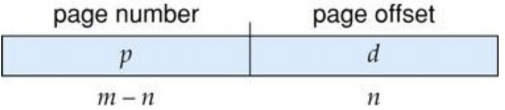
\includegraphics[scale=0.40]{numberoffset.png}
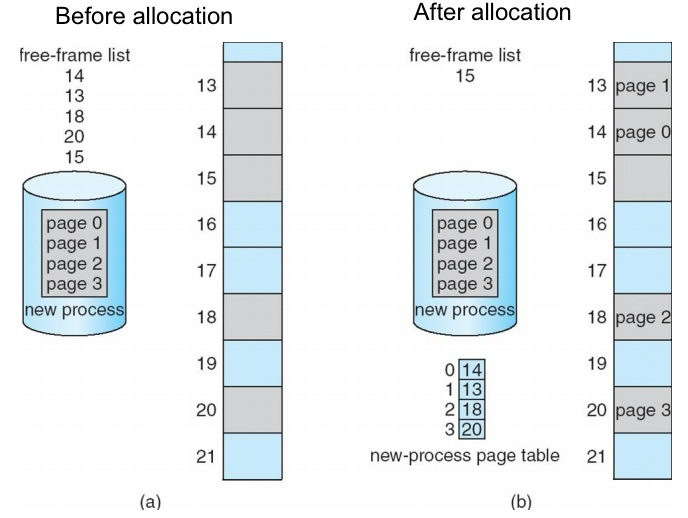
\includegraphics[scale=0.50]{paging1.png}
\caption{Paging}
\end{figure}


Bei der Auswahl der Pagegröße muss auf folgenes geachtet werden:
\begin{itemize}
\item Fragmentation
\item Table size
\item I/O overhead
\item Locality
\end{itemize}

\subsection{Assoziativspeicher}
\begin{itemize}
\item TLB = Assoziativer Cache für Adressübersetzungen.
\item Assoziativspeicher findet mit Hilfe paralleler Suche die translation(p,d)
\begin{itemize}
\item Wenn p im Assoziativregister: Besorge die Framenumber
\item Ansonsten hole die Framenumber vom Pagetable im Speicher
\end{itemize}
\end{itemize}
\begin{figure}[ht]
\centering
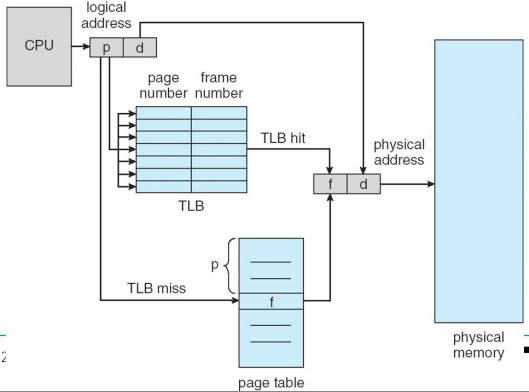
\includegraphics[scale=0.40]{tlb.png}
\end{figure}


>> Implementierung von PageTables ausgelassen<<
\subsubsection{Effective Access Time (EAT)}
\begin{itemize}
\item Assoziative Suche dauert $\tau$ Zeiteinheiten (z.B 1 ns)
\item Annahme: Ein Speicherzyklus dauert $\mu$ Zeiteinheiten (z.B 300 ns)
\item Hit-ratio $\alpha$, Anzahl der gefundene Pagenummern im Assoziativregister (in Prozent). 
$EAT = (\tau + \mu)  \alpha + (\tau + 2\mu) (1-\alpha) = \tau +2\mu - \mu\alpha$
\end{itemize}

\subsubsection{TLB Coverage}
\begin{itemize}
\item TLB Reach - Menge an Speicher, die für den TLB zugänglich sind
\item TLB Rech = (TLB Size) x (Page Size)

\item Erhöht die Page Size -> kann zu erhöhter Fragmentierung führen
\item Bietet multiple Page Sizes -> Programm können größere Page Sizes verwenden ohne erhöhte Fragmentierung zu riskieren
\end{itemize}

\subsection{Valid/Invalid Bit}
\begin{itemize}
\item Speicherschutz wird durch ein "`protection bit"' in jedem Frame erreicht
\item Jedem Eintrag im Page Table wird ein \textbf{Valid-invalid bit} angehängt
\begin{itemize}
\item valid deutet an, dass sich die im Zusammenhang stehende Page im logischen Adressraums des Prozesses befindet
\item invalid analog

\end{itemize}
\end{itemize}

\subsection{Shared Pages}
\subsubsection{Shared code}
\begin{itemize}
\item Eine Kopie von read-only Code wird unter Prozessen geteilt
\item Geteilter Code muss an der selben stelle im logischen Adressraum aller Prozesse auftauchen
\end{itemize}
\subsubsection{Shared Data}
\begin{itemize}
\item Daten mit Zeigern müssen an der selben Stelle im logischen Adressraum aller Prozesse auftauchen
\item Daten ohne  Zeige können überall im logische Adressraum sein
\item Synchronisation wird für konsistenten read/write Zugriff benötigt
\end{itemize}
\subsubsection{Private Code and Data}
\begin{itemize}
\item Jeder Prozess behält eine separate Kopie des Codes und der Daten
\item Pages für private Codes/Daten können überall im logischen Adressraum sein
\end{itemize}

\subsection{Page Table}
\subsubsection{Hierarchial Paging}

\begin{itemize}
\item Aufbrechen des logischen Adressraumes in viele page tables
\item Einfachstes Beispiel, two-level page table:
\begin{itemize}
\item Eine 32-bit große logische Adresse mit 1K page size wird unterteilt in
\begin{figure}[ht]
\centering
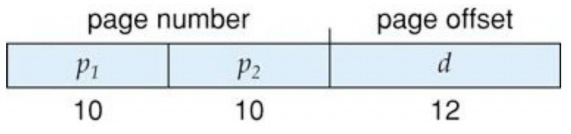
\includegraphics[scale=0.3]{twolevelpage.png}
\caption{Two Level Paging}
\end{figure}

\end{itemize}

\begin{figure}[ht]
\centering
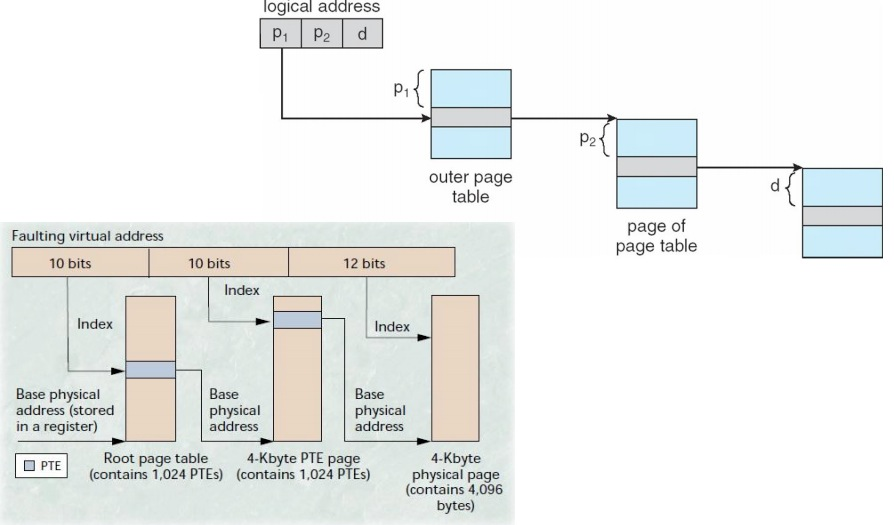
\includegraphics[scale=0.4]{topdownadress.png}
\caption{Top-Down Address-Translation Scheme}
\end{figure}

\begin{figure}[ht]
\centering
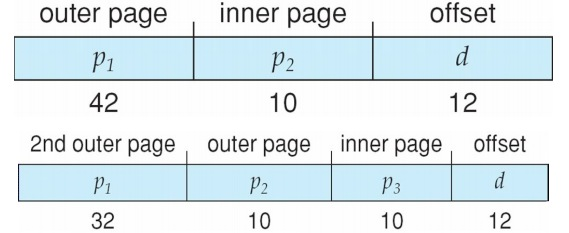
\includegraphics[scale=0.3]{topdownthreelevel.png}
\caption{Top-Down three-Level Paging Scheme}
\end{figure}

\end{itemize}

\subsubsection{Hashed Page Tables}
\begin{itemize}
\item Üblich in Adressräumen der größe > 32 bits
\item Die virtuelle Pagenummer wird in einen Pagetable gehashed. Dieses Pagetable beinhaltet ein eKette an Elementen, die alle an die selbe Stelle gehashed wurden.
\item Virtuelle Pagenummern werden mit den Elementen der Kette auf Gleichheit überprüft. Wenn eine Übereinstimmung gefunden wurde, wird der entsprechende physische Frame entnommen.
\end{itemize}

\subsubsection{Inverted Page Tables}
\begin{itemize}
\item Ein Eintrag pro echter Page im Speicher
\item Entry consists of the virtual address of the page stored in that real 
memory location, with information about the process that owns that 
page < Fuck this shit, not gonna translate it
\item Reduziert den benötigten Speicher für ein page table, erhöht jedoch die Zeit um den Table zu finden

\end{itemize}
\chapter{05bMemoryManagement - Cache Management}
\section{Basics}
\subsection{Operationen}
\begin{figure}[ht]
\centering
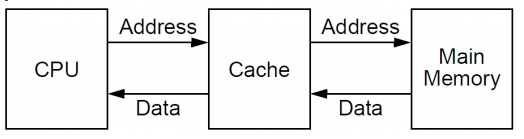
\includegraphics[scale=0.4]{operation.png}
\end{figure}

\begin{itemize}
\item Pufferspeicher zur Ausnutzung zeitlicher und räumlicher Lokalität
\item Niedrige Latenz, hohe Bandbreite 
\item Zugriffe auf den Hauptspeicher verringern
\item Puffer für asynchrone geprefetchte Operationen
\end{itemize}

\subsection{Zugriff}

\begin{itemize}
\item Cache miss
\begin{itemize}
\item \textit{Compulsory} (Cold Start, first reference) - Datenblock wurde zuvor nicht gecached
\item \textit{Capacity} - Die benötigten Daten passen nicht all in den Cache
\item \textit{Conflict} (collision, interference) - Abhängig von der Organisation könnten Daten miteinander in Konflikt geraten
\end{itemize}
\item Cache hit
\item Hit ratio
\end{itemize}

\begin{description}
\item[Neuman Architektur]\ \\ Befehle und Operanden liegen im selben Speicher. CPU braucht daher 2 Lesezyklen.
\item[Harvard Architektur]\ \\ Befehle und Operanden in jeweils unterschiedlichen Speichern. Ermöglicht gleichzeitiges Lesen von Befehl und Operanden
\item[Gemischter oder modifizierter Harvard]\ \\Separater Cache für Befehl und Operanden, aber selber Hauptspeicher
\end{description}

\begin{figure}[ht]
\centering
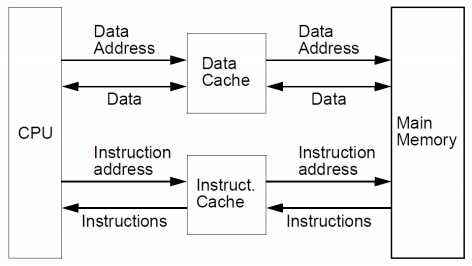
\includegraphics[scale=0.4]{modifiedharvard.png}
\caption{modifizierte Harvard Architektur}
\end{figure}

\begin{itemize}
\item Im Cache wird mit Hilfe von Hashing oder dem Vergleichen von Adressen gesucht.
\item Write Policies:
\begin{itemize}
\item Cache Hit
\begin{itemize}
\item \textbf{write-through}: Hauptspeicher immer auf dem neusten Stand, Schreiben braucht dafür seine Zeit.
\item \textbf{write-back}: Daten werden nur in den Cache geschrieben, der Hauptspeicher ist daher in einem temporär inkonsistenten Zustand.
\end{itemize}
\item Cache Miss
\begin{itemize}
\item \textbf{write-allocate}: Zu schreibende Daten werden vom Hauptspeicher in den Cache eingelesen. Geschrieben wird danach nach der vorliegenden "`write policy"'
\item \textbf{write-to-memory}: Es werden nur im Hauptspeicher Veränderungen vorgenommen.
\end{itemize}
\end{itemize}
\end{itemize}

\subsection{Cacheorganisation}
\begin{itemize}
\item \textbf{Voll Assoziativ}
\begin{itemize}
\item Jeder Speicherzeile kann mit jeder Cachezeile in Verbindung gebracht werden
\item Adressen im Cache werden via Hashing gefunden
\end{itemize}
\item \textbf{Direktes Mapping}
\begin{itemize}
\item Eine page befindet sich im Cache mit allen ihren Zeilen
\item Adressen im Cache werden via Vergleich gefunden
\end{itemize}
\item \textbf{N-way set Assoziativ}
\begin{itemize}
\item n pages befindet sich im Cache
\item Um eine Adresse im Cache zu finden werden n Vergleiche benötigt
\end{itemize}
\item Cache Zeilen mit fixer Länge (z.B 32/64 Bytes)
\item Adressen werden auf die Cachezeilen abgebildet
\item Daten werden durch ihr \textit{tag-field} identifiziert. Tags repräsentieren die Adresse des Datums im Speicher
\end{itemize}

\subsection{Hash Algorithmen}
\begin{itemize}
\item Modulo Hashing z.B  0. bis 5. bits als byte offset innerhalb der Cachezeile. 6. bis 18. bits um die Cachezeile auszuwählen und 19. bis 31. Bit als tag
\item Nehme zufällig gewählte Abschnitte der Adresse um die Cachezeile zu bestimmen. Wird nicht benutzt, da suboptimales Abbilduen von Adressen auf Cachezeilen.
\end{itemize}

\subsection{Synchronisation von Cache und Speicher}
\begin{description}
\item[Leeren des Caches] \ \\ Stellt Konsitenz sicher. Validiert Speicher indem es modifizierte Cachezeilen zurückschreibt und leert Cache
\item[Ungepufferte Operationen] \ \\ Benötigt z.B für Speichergemappte Register von I/O Geräten. 
\end{description}
\subsection{Cache Leistung}
\begin{itemize}
\item Bei Temporärer Lokalität wird eine \textit{write-back} Strategie bevorzugt.
\item Bei kleinen Caches  wird eien set-assoziative Implementierung mit großen Sets genommen.
\item Räumliche Lokalität bevorzugt lange Zeilen
\item Leistungssteigerung hängt vom Betriebssystem ab
\end{itemize}

\subsection{Cache Design Parameter}
\begin{itemize}
\item Größe
\item Zeilenlänge
\item Setgröße
\item Verwendung von virtuellen oder physikalische Adressen für Tagging/Indizierung
\item Austauschstrategie
\item Nutzung von \textit{write-allocate}
\item \textit{Write-through} oder \textit{write-back}

\end{itemize}
\subsection{Cache Anordnung}
\begin{itemize}
\item Länge der Cachezeilen hat Einfluss auf die Datenstruktur
\item \textit{Problem}: Mehrfache Misses werden durch "`nicht-angeordnete"' Datenstrukturen die mehrere Cachezeilen umfassen verursacht.
\item \textit{Lösung}:  Struktur wird zu einem mehrfachen der Zeilenlänge aufgefüllt

\begin{figure}[ht]
\centering
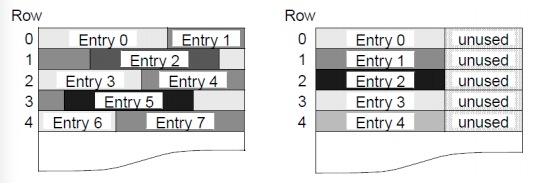
\includegraphics[scale=0.4]{cachealignment.png}
\end{figure}

\item In der Praxis treten Cacheanordnungs Probleme kaum auf
\item Einträge sind Blöcke. Speicher wird Blockweise vom Speicher in den Cache kopiert
\item Daraus folgt: Wenn Block = Zeile, sind die Zeilen voll
\end{itemize}

\subsection{Index und Tags}
\begin{itemize}
\item Adressen im Cache werden mit Hilfe eines Index gefunden, welcher der Zeilennummer entspricht
\item  Tag bestimmt ob ein Speicherblock von der CPU benötigt wird.
\item  CPUs benutzen oft virtuelle Adressen
\end{itemize}

\section{Virtuell indizierter, virtuell getaggter Cache (VIVT)}
\begin{itemize}
\item Kein MMU Zugriff benötigt für Cachezugriff
\item Alte ARM Architektur
\end{itemize}

\begin{figure}[ht]
\centering
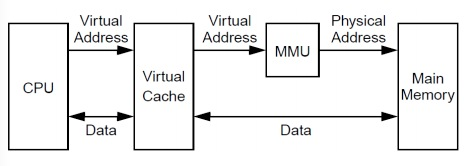
\includegraphics[scale=0.4]{VIVT.png}
\end{figure}

MMU sitzt hinter dem Cache, jedoch nur virtuell/virtuell Möglich.

\begin{itemize}
\item \textbf{Ambiguity Problem}: Zwei identische virtuelle Adressen zeigen auf unterschiedliche physikalische Adressen zu zwei verschiedenen Zeitpunkten
\item \textbf{Alias Problem}: Unterschiedliche virtuelle Adressen zeigen auf die selbe physikalische Speicherstelle
\end{itemize}

\begin{description}
\item \textbf{Context Switch} \ \\ Cache muss geleert werden, da identische virtuelle Adresse von unterschiedlichen Adressräumen auf unterschiedliche physikalische Adressen weisen können (und mit hoher wahrscheinlichkeit auch tun werden)

\item \textbf{fork()} \ \\Das Kind benötigt eine komplette Kopie des Elterns Adressraum.
\item \textbf{exec()} \ \\ leert Cache um amibguities zu verhindern. Wird nicht beim Zurückschreiben benötigt, da der Speicher eh überschrieben wird.

\item \textbf{exit()} \ \\ leert den Cache
\item \textbf{brk() and sbrk()} \ \\ "`Growing"' benötigt keine Aktion, "`shrinking"' benötigt selektive Cache leerung.
\end{description}

\subsection{Shared Memory und Memory mapped files}
\begin{itemize}
\item Das Problem mit  Aliases ist, dass mehr virtuelle Adressen benutzt werden um auf die selben pysikalischen Speicherstellen zu verweisen
\item Also: Nicht erlauben und nicht cachen.
\item Erlaube nur adressen die auf die selbe Cachezeile mappen (wenn der Cache direkt gemapped und write-allocate verwendet)
\item Jeder Frame ist von exakt einer virtuellen Adresse zu jedem Zeitpunkt erreichtbar
\end{itemize}

 Gepufferte I/O machen keine Probleme, Ungepufferte hingegen schon, da:
 \begin{itemize}
 
\item Schreiben: Information könnten immer noch im Cache sein
\item Lesen: Cache muss geleert werden
 \end{itemize}

\subsection{User-Kernel Data Ambiguities (Doppeldeutigkeit,Missverständnis)}
\begin{itemize}
\item Schreibe Systemdateien zurück bevor man in den usermode zurück kehrt.
\item Cache leeren before man in den user mode zurück kehrt
\end{itemize}

\subsection{Echzeit Charakteristik}

\begin{itemize}
\item Schnell da die MMU nur bei Cache Misses benötigt wird
\item Konstante  Ausführungszeit eines Prozesses mit festem Speichermapping
\item Variable Ausführungszeit im Falle von dynamischer Speicherallokierung (werden durch conflict misses ausgelöst, wenn ein voller Assoziativcache verwendet wird)
\item Teure Kontextwechsel und I/O da der Cache geleert werden muss
\end{itemize}

\section{Virtuell indizierter, physikalisch getaggter Cache(VIPT)}
\begin{itemize}
\item MMU Zugriff benötigt
\item Intel Core++ Prozessor
\item Instruktions Cache ARM Cortex

\begin{figure}[ht]
\centering
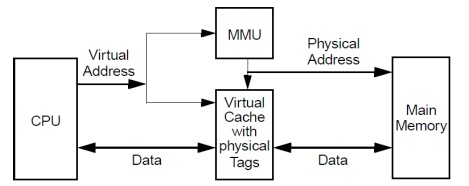
\includegraphics[scale=0.5]{VIPT.png}
\end{figure}

\item Wird oft als first-level Cache verwendet (z.B UltraSPARC II)
\item \textbf{Cache Management}
\begin{itemize}
\item Keine Mehrdeutigkeiten
\item Keine Cacheleerung bei Kontextwechsel
\item Virtuelle Startadressen müssen auf die selbe Cachezeile gemapped sein
\end{itemize}

\item Es könnten Konflike entstehen wenn Datenstrukturen, der Abstand der Adressen ein Vielfaches der Cachegröße beträgt auf die selbe Cachezeile gemapped sind. Dies kann durch n-way caching behoben werden.
\end{itemize}
\subsection{Laufzeit Eigenschaften}
\begin{itemize}
\item Schnelle Kontextwechsel, Interrupt-handlig und System Calls, da Cache flushes die meiste Zeit verhindert werden
\item Verzögerte Write-Back nach einem Kontextwechsel. 
\item Unterschiedliche Ausführungszeit im Falle von dynamischem Speichermanagement, welche durch Conflict misses verursacht werden
\item  Variable Suchdauer, welche durch die Adressübersetzung der MMU verursacht wird.
\item Problematik bei multiprozessor Systemen mit shared memory: Welche Zeile leeren?
\end{itemize}


\section{Physikalisch indizierter, physikalisch getaggter Cache (PIPT)}

\begin{itemize}
\item Daten Cache ARM Cortex
\end{itemize}

\begin{figure}[ht]
\centering
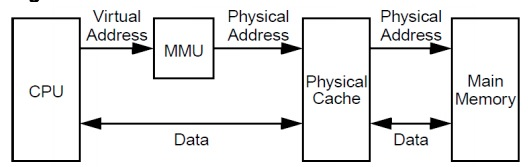
\includegraphics[scale=0.5]{PIPT.png}
\end{figure}

\textbf{Vorteile}
\begin{itemize}
\item Komplett transparent für den Prozessor
\item Keine Unterstützung für Performanz-kritische Systeme benötigt.
\item SMP mit shared memory kann ein in der Hardware implementiertes Kohärenzprotokoll benutzen
\end{itemize}
\section{Physikalisch indizierter, virtuell getaggter Cache (PIVT)}
\begin{huge}
\textbf{>>>>>>SINNLOS!<<<<<<} 
\end{huge}
\begin{small}
Daher nicht praktiziert...
\end{small}

\section{Page Conflicts}

Werden durch zufällige Allokierungen von physikalischem Speicher verursacht

\begin{figure}[ht]
\centering
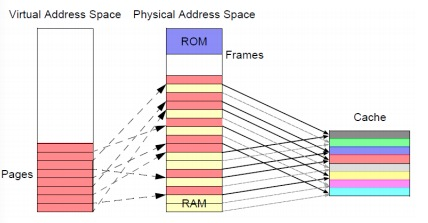
\includegraphics[scale=0.5]{pageconflict.png}
\end{figure}
 \ \\
Angrenzend virtueller Speicher wird normallerweise auf beliebig freie physikalische pages abgebildet.

\subsection{Page Colouring}
Problem von zufälliger Page Färbung : Benachbarte Codes/Daten könnten nicht auf den selben Cache abgebildet werden, wenn sie auf die selbe Zeile hashen.

Lösung1: 

\begin{itemize}
\item Folgen von zufälligem page coloring:
\begin{itemize}
\item Cache Conflicts
\item Cache nur teilweise benutzt
\item Signifikante unterschiede in der Laufzeit \\
$X(p \in bin) = {P \choose p} (\frac{1}{C})^p(1-\frac{1}{C})^{P-p} $
P: Anzahl von allokierten Pages
p: p pages die der selben Cachezeile entsprechen
C: Nummer der Farbe
\end{itemize}
\end{itemize}


\subsection{Cache Konflikte vermeiden}
\subsubsection{Cachepartitionierung}
\begin{itemize}
\item Unterteile den physikalischen Speicher in disjunkte  Teilmengen. Alle Pages einer Teilmenge werden auf die selbe Cachepartition abgebildet.\\
\textit{Beispiel:} \\
\item Alle roten und blauen Pages fürs Betriebssystem
\item Alle gelben Pages für die echtzeit Anwendung
\item Alle grünen Pages für die Hintergrundprozesse.
\end{itemize}


\begin{figure}[ht]
\centering
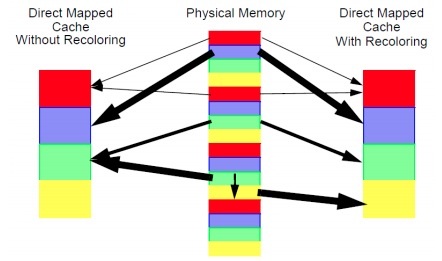
\includegraphics[scale=0.5]{pagecoloring.png}
\caption{Analyse von Zugriffsmustern und Page coloring}
\end{figure}


\chapter{05cMemoryManagement}
\chapter{06aFileSystems}

\section{Das Konzept von Dateien}
\begin{itemize}
	\item Ziel: Moeglichkeit, große Mengen von Daten zu speichern
	\item Datei: Zusammenhaengender logischer Adressraum
	\item Dateitypen
		\begin{itemize}
			\item Daten: Numerisch, character, binaer
			\item Programm
		\end{itemize}
	\item Speichern von Daten und Programmen
		\begin{itemize}
			\item Persistent
			\item Konsistent: Berechenbare Verhalten beim gleichzeitigem Zugriff
		\end{itemize}
	\item Nach vorher gespeicherten Daten sehen
\end{itemize}

\section{Dateisysteme}
\begin{itemize}
	\item OS soll Unordnung auf physikalischen Geraeten verbergen
		\begin{itemize}
			\item Low-level device control (Lesen veranlassen, etc.)
			\item High-level abstractions (Datei lesen, etc.)
		\end{itemize}
	\item U.u. ermoeglicht OS unterschiedlichen Level von Zugriffen fuer unterschiedliche Programme
		\begin{itemize}
			\item Physical disk (surface, cylinder, sector)
			\item Logical disk = partition (disk block\#)
			\item Logical volume = multiple partitions (volume block\#)
			\item Logical file (file block, record, byte\#)
		\end{itemize}
\end{itemize}

\section{Festplatten}
\begin{itemize}
	\item Stapel von Platten, welche sich mit 3.600-15.000 RPM drehen
	\item Arme rotieren um den Drehpunkt, Koepfe lesen und schreiben
	\item Platten sind in konzentrische Tracks aufgeteilt
	\item Ein Stack mit Tracks fester Groeße ist ein Zylinder
	\item Meistens nur ein Kopf gleichzeitig aktiv
	\item Zugriffszeit besteht aus zwei Komponenten
		\begin{itemize}
			\item Seek time: Zeit, die die Platte braucht, um den Kopf zu dem entsprechenden Zylinder zu bewegen
			\item Rotational delay: Zusaetzliche Zeit, die die Platte braucht, um den entsprechenden Sektor zum Kopf zu bewegen
		\end{itemize}
\end{itemize}

\begin{figure}[ht]
\centering
\includegraphics[scale=0.3]{harddisk.png}
\caption{Zylinder, Tracks und Sektoren}
\end{figure}
\subsection{Das Positionierungssystem}
\begin{itemize}
	\item Suche besteht aus 4 Phasen
		\begin{itemize}
			\item speedup - Auf Hoechstgeschwindigkeit beschleunigen (oder die Haelfte)
			\item coast - Hoechstgeschwindigkeit bei langen Suchen
			\item slowdown-stops - Arm nahe dem Ziel
			\item settle - Kopf auf entsprechenden Track legen
		\end{itemize}
	\item Sehr kurze Suchen haengen von settle time ab (1 ms)
	\item Kurze Suchen (200-400 cyl.) haengen von speedup ab
\end{itemize}

\subsubsection{Details zur Suche}
\begin{itemize}
	\item Kopf wechselt vergleichsweise zu kurzen Suchen (hae?)
		\begin{itemize}
			\item Moeglicherweise muss der Kopf angepasst werden
			\item Ansetzen dauert beim Schreiben laenger als beim Lesen
			\item Weicht das Lesen vom Track ob, wird mit Checksumme Fehler erkannt und es wird erneut versucht
			\item Kommt man beim Schreiben vom Track ab, zerstoert man einen anderen
		\end{itemize}
	\item Disk speichert Tabelle mit Drechachsenmotorleistung
		\begin{itemize}
			\item Bildet Distanz auf Leistung und Zeit ab
			\item Disk erweitert Eintraege
			\item Tabelle wird gesetzt von periodischer thermischeir Rekalibrierung (hae?)
		\end{itemize}
\end{itemize}

\subsection{Sektoren}
\begin{itemize}
	\item Disk-Schnittstelle gibt lineares Array von Sektoren (LBA)
	\item Disk bildet logische Sektoren \#s auf physikalische Sektoren ab (CHS)
		\begin{itemize}
			\item Zoning: Mehr Sektoren auf laengere Tracks packen
			\item Track skewing: Sektor 0 Position haengt vom Track ab
			\item Sparing: Fehlerhafte Sektoren werden woanders hingemapt
		\end{itemize}
	\item OS kennt nicht logisches (LBA) oder physikalisches Sektor (CHS) mapping
		\begin{itemize}
			\item Große Unterschiede in der logischen Sektorenanzahl verlaengern Suche
			\item Hoechst nichtlineare Beziehung
			\item OS weißt nichts von Rotationspositionen
			\item Kann epirisch Tabelle bilden um Zeit abzuschaetzen
		\end{itemize}
\end{itemize}

\subsection{Disk Schnittstelle}
\begin{itemize}
	\item Kontrolliert HW, vermittelt Zugriffe
	\item Computer und Disk oft durch Bus verbunden (z.B. SATA)
		\begin{itemize}
			\item U.u. viele Geraete ein einem Bus
			\item Ggf. Geraete ueber Netz verbunden (z.B. SAN)
		\end{itemize}
	\item Disk/Schnittstellen features
		\begin{itemize}
			\item Trennen vom Bus waehrend Anfragen
			\item Warteschlange fuer Befehle: Mehrere Anfragen, kann geschedulet werden
			\item Vorauslesen in den Cache, sonst wuerden ganze Umdrehungen pro sequentielles Lesen gebraucht
			\item Cache fuers Schreiben
		\end{itemize}
\end{itemize}

\begin{figure}[ht]
\centering
\includegraphics[scale=0.4]{san.png}
\caption{SAN}
\end{figure}

\subsection{Disk Leistung}
\begin{itemize}
	\item Das Setzen und Ordnen von Anfragen ist ein großes Problem
		\begin{itemize}
			\item Sequentielle I/O wesentlich schneller als zufaellige
			\item Lange Suchen wesentlich langsamer als kurze
			\item Strom kann wegfallen, dann inkonsistenter Zustand
		\end{itemize}
	\item Vorsicht bei Reihenfolge zur Wiederherstellung
	\item Moeglichst zusammenhaegende Zugriffe
	\item Versuche, Anfragen zu sortieren, um seek times gering zu halten
\end{itemize}

\section{SSDs}
\begin{itemize}
	\item Komplett stabiler Zustand, keine bewegenden Teile
		\begin{itemize}
			\item Speichert Daten in Form von Ladungen
			\item Weniger Stromverbrauch und Hitze
			\item Keine mechanischen Suchzeiten
		\end{itemize}
	\item Beschraenkte Anzahl an Ueberschreibungen
		\begin{itemize}
			\item Bloecke nutzen nach 1.000-100.000 Loeschungen ab
			\item Brauch flash translation layer (FTL), damit wiederholtes Schreiben auf logischen Block nicht physikalischen Block abnutzt
			\item FTL kann Performance stark beeinflussen
			\item Zufaelliges Schreiben teuer
		\end{itemize}
	\item Limitierte Haltbarkeit
		\begin{itemize}
			\item Ladung nimmt ab
			\item Ausschalten fuer ein Jahr kann Datenverlust hervorrufen
		\end{itemize}
\end{itemize}

\subsection{Typen von Flash-Speichern}
\begin{itemize}
	\item NAND flash (meistens anzutreffen)
		\begin{itemize}
			\item Hoehere Dichte
			\item Schnelles Loeschen und Schreiben
			\item Mehr interne Fehler $\Rightarrow$ Fehlerbehebung erforderlich
		\end{itemize}
	\item NOR flash
		\begin{itemize}
			\item Schnelleres Lesen bei kleinen Dateneinheiten
			\item Kann direkt ausgefuehrt werden
			\item Signifikant langsameres Loeschen
		\end{itemize}
	\item Single-level cell (SLC) vs. Multi-Level cell (MLC)
		\begin{itemize}
			\item MLC codiert viele Bits
			\item MLC langsamer als SLC
		\end{itemize}
\end{itemize}

\subsection{NAND flash Uebersicht (Uebliches Geraet)}
\begin{itemize}
	\item Hat 2112-byte Seiten (2048 Bytes Daten + 64 Bytes Metadaten \& ECC)
	\item Block hat 64 (SLC) oder 128 (MLC) Seiten
	\item Blocks in 2-4 Ebenen (planes) unterteilt
	\item Kann eine Seite auf einmal lesen
	\item Muss kompletten Block loeschen, bevor dieser ueberschrieben werden kann (teuer)
\end{itemize}

\begin{figure}[ht]
\centering
\includegraphics[scale=0.3]{ssd.png}
\caption{SSD Logik}
\end{figure}

\subsection{SSD Performance Optimierung}
\begin{itemize}
	\item Freie Bloecke
		\begin{itemize}
			\item SSD Controller haelt immer eine Menge von freien Blocken
			\item Bei eine re-write wird freie Block zum Schreiben benutzt, alter wird freigegeben
			\item Loeschen findet im Hintergrund statt, wenn SSD nichts zu tun hat
		\end{itemize}
	\item trim Befehl
		\begin{itemize}
			\item OS gibt SSD controller unbenutzte logische Bloecke an
			\item Diese muessen bei eine re-write nicht kopiert werden
			\item Sie erhoehen den Pool der freien Bloecke nach gargabe collection
		\end{itemize}
\end{itemize}

\chapter{06bFileSystems}

\section{Dateien}
\begin{itemize}
	\item Eine Datei ist eine Sammlung von Informationen
		\begin{itemize}
			\item Ausfuehrbares Programm
			\item Textdateien
			\item Komprimierte Binaer-images
			\item Strukturierte Dokumente
		\end{itemize}
	\item Eine Datei hat eine Menge von Attributen (sprich (OS) meta data)
	\item Attribute haengen von OS und FS ab, z.B.
		\begin{itemize}
			\item Name, ID
			\item TypSSD Logik
			\item Ort (physikalische Adresse auf Geraet)
			\item Groeße (Anzahl Bytes oder Blocks)
			\item Schutz (wer kann wie zugreifen)
		\end{itemize}
\end{itemize}

\begin{figure}[ht]
\centering
\includegraphics[scale=0.25]{file_attributes.png}
\caption{Typische Dateiattribute}
\end{figure}

\subsection{Dateistruktur 1}
\begin{itemize}
	\item Keine - Sequenz von Woertern/Bytes
	\item Simple record Struktur
		\begin{itemize}
			\item Zeilen
			\item Feste Laenge
			\item Variable Laenge
		\end{itemize}
	\item Kompexe Struktur
		\begin{itemize}
			\item Formattiertes Dokument
			\item Verschiebbares ausfuehrbares Objekt
		\end{itemize}
\end{itemize}

\subsection{Dateistruktur 2 (OS Ansicht)}

\begin{figure}[ht]
\centering
\includegraphics[scale=0.3]{file_structure.png}
\caption{Datei Struktur}
\end{figure}

\begin{itemize}
	\item Drei Arten von Dateien
		\begin{itemize}
			\item Byte Sequenz (ermoeglicht maximale Flexibilitaet)
			\item record Sequenz (haeufig mit fester Groeße)
			\item Baum (manchmal mit variabler Groeße)
		\end{itemize}
\end{itemize}

\subsection{Dateitypen}
\begin{itemize}
	\item Regulaere Dateien: ausfuehrbar, dll, object, source, text
	\item Spezielle Dateien: Ordner, Geraete (character, block), Links
	\item Dateityp kann an folgenden Stellen stehen:
		\begin{itemize}
			\item interne Sturktur im FS (z.B. Unix): Inode
			\item Nmane (z.B. Dateinamenserweiterungen in Windows): .com, .exe..
			\item Inhalt (z.B. Unix, media files): Magic number oder initial character (z.B. \#! fuer Shellscripts)
		\end{itemize}
\end{itemize}

\begin{figure}[ht]
\centering
\includegraphics[scale=0.3]{regular_filetypes.png}
\caption{Regulaere Dateitypen 1}
\end{figure}

\begin{figure}[ht]
\centering
\includegraphics[scale=0.4]{regular_filetypes2.png}
\caption{Regulaere Dateitypen 2}
\end{figure}

\subsection{Abstrakte Dateioperationen}
\begin{itemize}
	\item create()
	\item write()
	\item read()
	\item reposition() (innerhalb einer Datei)
	\item delete()
	\item truncate()
	\item open($F_i$): suche in Ordnerstruktur nach $F_i$ und bewege die Metadaten in den Speicher
	\item close($F_i$): bewege gecachte Metadaten von Eintrag $F_i$ im Speicher in die Ordnerstruktur
\end{itemize}

\begin{figure}[ht]
\centering
\includegraphics[scale=0.4]{filesystem_interaction.png}
\caption{Interaktionen zwischen einem Programm und dem Dateisystem}
\end{figure}

\subsection{Ziele der Dateiverwaltung}
\begin{itemize}
	\item Liefer ueberzeugendes Namenschema fuer Dateien
	\item Liefer einheitlichen I/O Support fuer unterschiedliche Speichergeraetetypen
	\item Liefer standardisierte Menge an I/O Schnittstellenfunktionen
	\item Minimiere Verlust oder Verfaelschung von Dateien
	\item Liefer I/O Support und Zugriffskontrolle fuer mehrere Benutzer
	\item Erweiter Systemadministration (z.B. Backup)
	\item Liefer akzeptierbare Performance
\end{itemize}

\subsection{Dateinamen}
\begin{itemize}
	\item Textuelle Namen
	\item Eingeschraenktes Alphabet
		\begin{itemize}
			\item Nur bestimmte characters
			\item Eingeschraenkte Laenge
			\item Case (in)sensitive
		\end{itemize}
	\item Nur bestimmte Formate, z.B.
		\begin{itemize}
			\item DOS: 8 character string.xyz character suffix
			\item XP: 255 character string.xyz character suffix
		\end{itemize}
	\item Namen mussen bestimmte weitere Eigenschaften einhalten, z.B. Erweiterungen xyz.c, wenn der C-Compiler laufen soll
\end{itemize}

\subsection{Oeffnen von Dateien}
Unterschiedliche Metadaten werden gebraucht, um das Oeffnen von Dateien zu verwalten
\begin{itemize}
	\item file pointer: Zeiger auf die letzte Lese-/Schreibaktion, pro Prozess, der die Datei offen hat
	\item access rights: Pro Prozess/Task gibt es Zugriffsinformationen
	\item file-open count: Zaehler, welcher angibt, wie oft die Datei offen ist, um Entfernen von Daten aus der Datei zu ermoeglichen, wenn der letzte Prozess beendet ist
	\item disk location: Cache mit Datenzugriffsinformationen
\end{itemize}

\subsection{Dateizugriff}
\begin{itemize}
	\item Strikt sequentieller Zugriff (fruehere Systeme)
		\begin{itemize}
			\item Lies alle Bytes von Anfang an
			\item Keine Spruenge moeglich, nur zurueck
			\item Ausreichend, solange Tapes benutzt wurden
		\end{itemize}
	\item Zufaelliger Zugriff (aktuelle System)
		\begin{itemize}
			\item Lies Bytes in beliebiger Reihenfolge
			\item Essenziell fuer Datenbankensysteme
		\end{itemize}
\end{itemize}

\subsubsection{Dateiorganisation und Zugriff}
Moegliche Zugriffsmuster:
\begin{itemize}
	\item Lies komplette Datei
	\item Lies individuelle Block einer Datei
	\item Lies Bloecke mit den folgenden oder vorangehenden
	\item Finde eine Untermenge an records wieder auf
	\item Schreibe/update eine komplette Datei sequenziell
	\item Einfuegen/Loeschen/Updaten eines records in einer Datei
	\item Update Bloecke in eine Datei
\end{itemize}

\subsubsection{Dateizugriffsmethoden}
\begin{itemize}
	\item Sequenzieller Zugriff
		\begin{itemize}
			\item read next
			\item write next
			\item rewind
			\item no read after last write
			\item append
		\end{itemize}
	\item Direkter Zugriff
		\begin{itemize}
			\item read n
			\item write n
			\item position to n
			\item read next
			\item write next
		\end{itemize}
	\item n = relative Position
	\item Einfache (unstrukturierte) Datei
		\begin{itemize}
			\item Einheit: Byte (manchmal Block)
			\item Will eine Applikation einen Datencontainer strukturieren moechte, so hat es die interne Struktur zu implementieren
		\end{itemize}
	\item Strukturierte Datei
		\begin{itemize}
			\item Einheit: record (oder user type object, ...)
		\end{itemize}
	\item Seit Unix bieten OSes nur noch plain file, Programme und Bibliotheken koennen darauf spezielle Strukturen implementieren
\end{itemize}

\begin{figure}[ht]
\centering
\includegraphics[scale=0.4]{sequential_access.png}
\caption{Ein sequenzieller Zugriff auf eine Datei}
\end{figure}

\subsubsection{Operationen auf unstrukturierten Dateien}
\begin{itemize}
	\item CreateFile(pathname)
	\item DestroyFile(pathname)
	\item OpenFile(pathname, read/write)
	\item ReadFile(FID, byte-range, memory location)
	\item WriteFile(FID, byte-range, memory location)
	\item CloseFile(FID)
	\item PositionPointer(FID, position for pointer)
\end{itemize}

memory location ist die data area im AS des aufrufenden Prozesses (z.B. im Heap oder Stack)

\subsection{Plain File}
\begin{itemize}
	\item Definition: Plain File ist eine Sequenz von Bytes, meisten auf der Disk
	\item Characteristic: Man kann auf jedes Byte in einer unstrukturierten Datei zugreifen, wenn der Zeiger richtig gesetzt ist
	\item Problem: Disks koennen nicht auf Bytes sondern nur auf Bloecke zugreifen
	\item Solution: Buffer file blocks (klassische Methode) oder ganze Dateien (auf den Speicher abgebildete Dateien) im Hauptspeicher
\end{itemize}

\subsection{Strukturierte Datei}

\begin{figure}[ht]
\centering
\includegraphics[scale=0.4]{structured_file.png}
\caption{Strukturierte Datei}
\end{figure}

\begin{itemize}
	\item Records = logische Einheiten streng an eine Applikation gebunden
	\item Records mit gleicher Groeße oder nicht
	\item Records mit einem speziellen Schluesselfeld ($\Rightarrow$ etwas Ordnung in der Datei)
\end{itemize}

\begin{figure}[ht]
\centering
\includegraphics[scale=0.4]{file_operation.png}
\caption{Datei Operation 1}
\end{figure}

\begin{figure}[ht]
\centering
\includegraphics[scale=0.4]{file_operation2.png}
\caption{Datei Operation 2}
\end{figure}

\section{Ziele von Ordnern}
\begin{itemize}
	\item Benennung: Praktisch fuer Benutzer
		\begin{itemize}
			\item Zwei Benutzer koennen den gleichen Namen fuer unterschiedliche Dateien benutzen
			\item Diesselbe Datei kann mehrere unterschiedliche Namen haben
		\end{itemize}
	\item Gruppierung: Logische Gruppen von Dateien
	\item Effizienz: Schnelle Operationen
\end{itemize}

\subsection{Operationen von Ordnern}
\begin{itemize}
	\item Datei erstellen
	\item Datei loeschen
	\item Datei umbenennen
	\item Dateisystem traversieren
	\item Ordnerinhalt auflisten
	\item Datei suchen
\end{itemize}








\chapter{07aImplementingFileSystems}
\chapter{07bImplementingFileSystems}
\chapter{08SecondaryStorageStructure}
\chapter{09IoSystems}

\end{document}
